\section{Results}\label{sec:results} 

In this section, we describe the results of our experiments.  We explore which
non-mainstream resolvers are available; how
the performance of mainstream resolvers compares to that of non-mainstream
resolvers; and whether (and to what extent) high encrypted DNS response time
correlates to large geographic distance or high network latency.

\subsection{Are Non-Mainstream Resolvers Available?}

\if 0
\begin{table}[t!]
\centering
\begin{tabular}{lllll}
\hline
\textbf{Location} & \textbf{Resolver} & \textbf{Responsive?} & & \\
    & & \textbf{Ohio} & \textbf{Seoul} & \textbf{Frankfurt} \\
\midrule
North America     & \begin{tabular}[c]{@{}l@{}}dnscrypt.ca-1-doh\\ dnscrypt.ca-2-doh\\ doh-cleanbrowsing\\ doh.post-factum.tk\end{tabular} & \begin{tabular}[c]{@{}l@{}}\\ \\ \\ \end{tabular} & \begin{tabular}[c]{@{}l@{}}\\ \\ \\ \end{tabular} & \begin{tabular}[c]{@{}l@{}}\\ \\ \\ \end{tabular}    \\ \midrule
Asia              & \begin{tabular}[c]{@{}l@{}}doh.tiarap.org\\ jp.tiarap.org\\ doh.linuxsec\end{tabular} & \begin{tabular}[c]{@{}l@{}}\\ \\ \end{tabular}      & \begin{tabular}[c]{@{}l@{}}\\ \\ \end{tabular}      & \begin{tabular}[c]{@{}l@{}}\checkmark\ \checkmark\ \end{tabular}            \\ \midrule
Europe            & \begin{tabular}[c]{@{}l@{}}doh.bortzmeyer\\ doh.appliedprivacy\\ doh.chewbacca.meganerd.nl\\ doh.powerdns\end{tabular} & \begin{tabular}[c]{@{}l@{}}\\ \\ \\ \end{tabular} & \begin{tabular}[c]{@{}l@{}}\\ \\ \\ \end{tabular} & \begin{tabular}[c]{@{}l@{}}\\ \\ \\ \end{tabular} \\ \bottomrule
\end{tabular}
\caption{Resolvers that failed to respond from each vantage point.}
\label{tab:unresponsive}
\end{table}
\fi

We first aimed to study the availability of encrypted DNS
resolvers---particularly non-mainstream resolvers. Our initial goal in doing
so was to better understand the extent to which the encrypted DNS resolvers
maintained on public lists were operating reliably.
We received responses from most resolvers that we queried.
Table~\ref{tab:unresponsive} shows the DoH resolvers that we failed to receive
a response from, and Table~\ref{tab:errors} shows the most common errors we
received from attempting to communicate with unresponsive resolvers.  The
results show that the most common errors from unavailable resolvers were
related to a failure to establish a TCP connection or a TLS session.
\AH{Review this previous sentence later with the full data} It is likely that
in many of these cases, the resolver itself was simply no longer operational;
additional longitudinal measurements could confirm this hypothesis.

\begin{figure}[t!]
\hspace*{-1in}
\begin{minipage}{1.35\textwidth}
    \subfigure[North America (Local).]{%
\label{fig:Ohio_NA}%
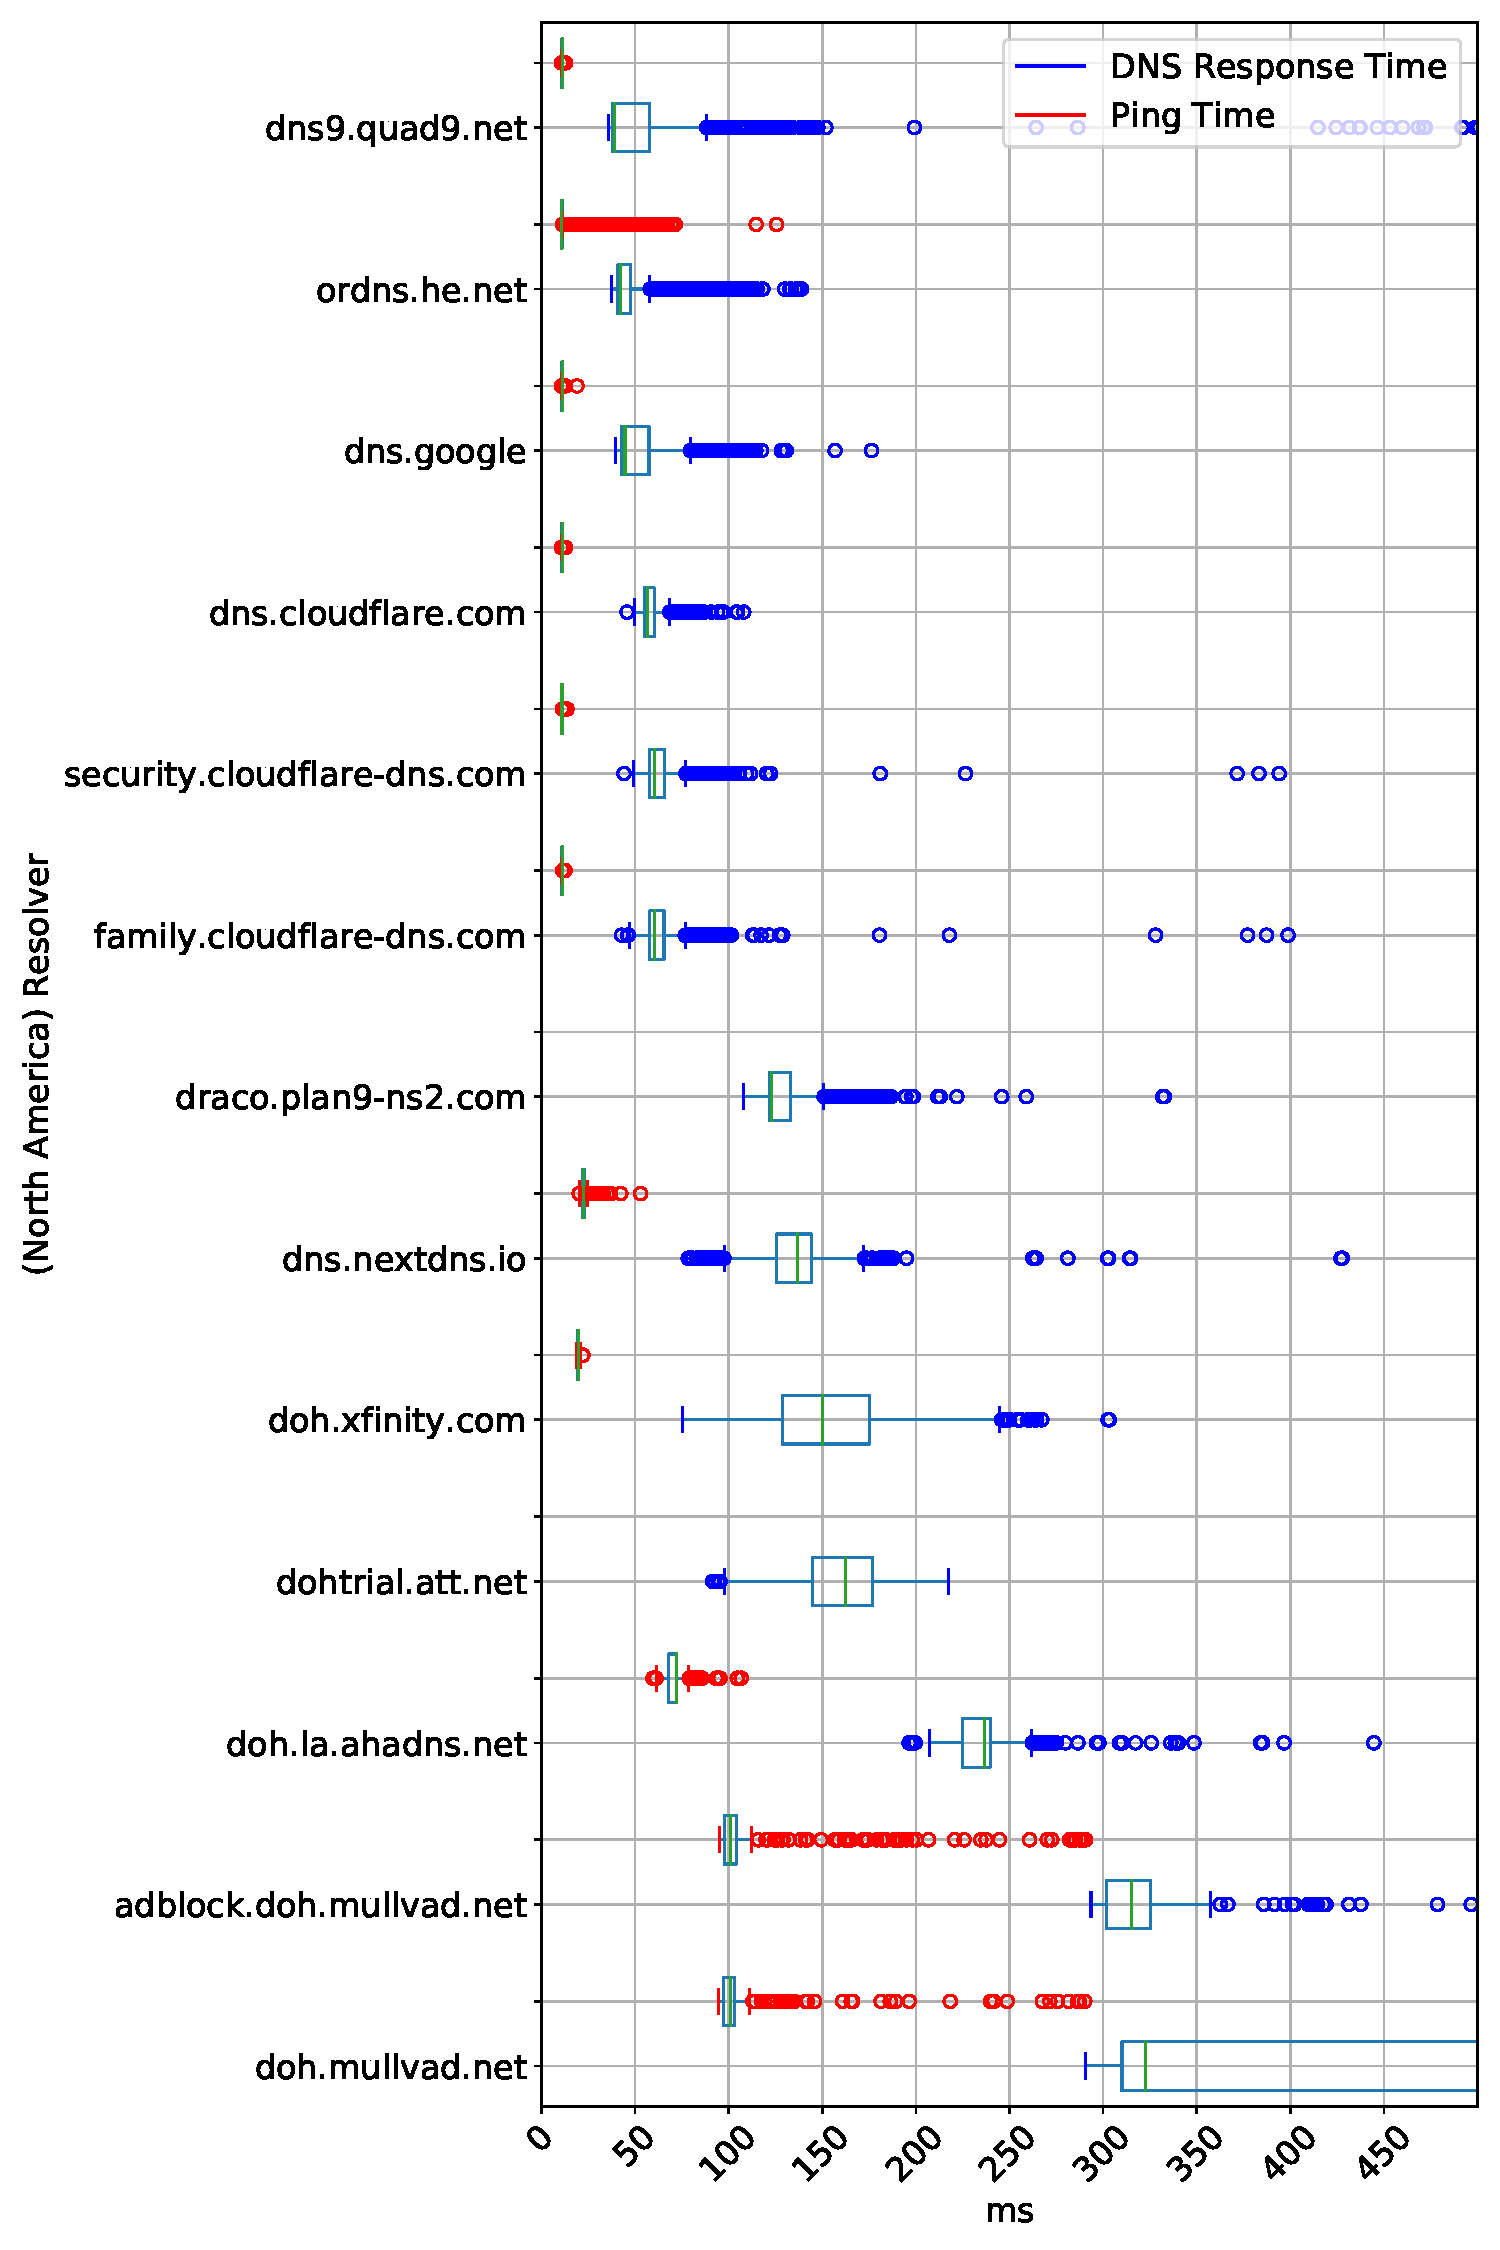
\includegraphics[width=0.32\linewidth]{figures/Ohio_North_America.pdf}}%
\hfill%
\subfigure[Asia.]{%
\label{fig:Ohio_Asia}%
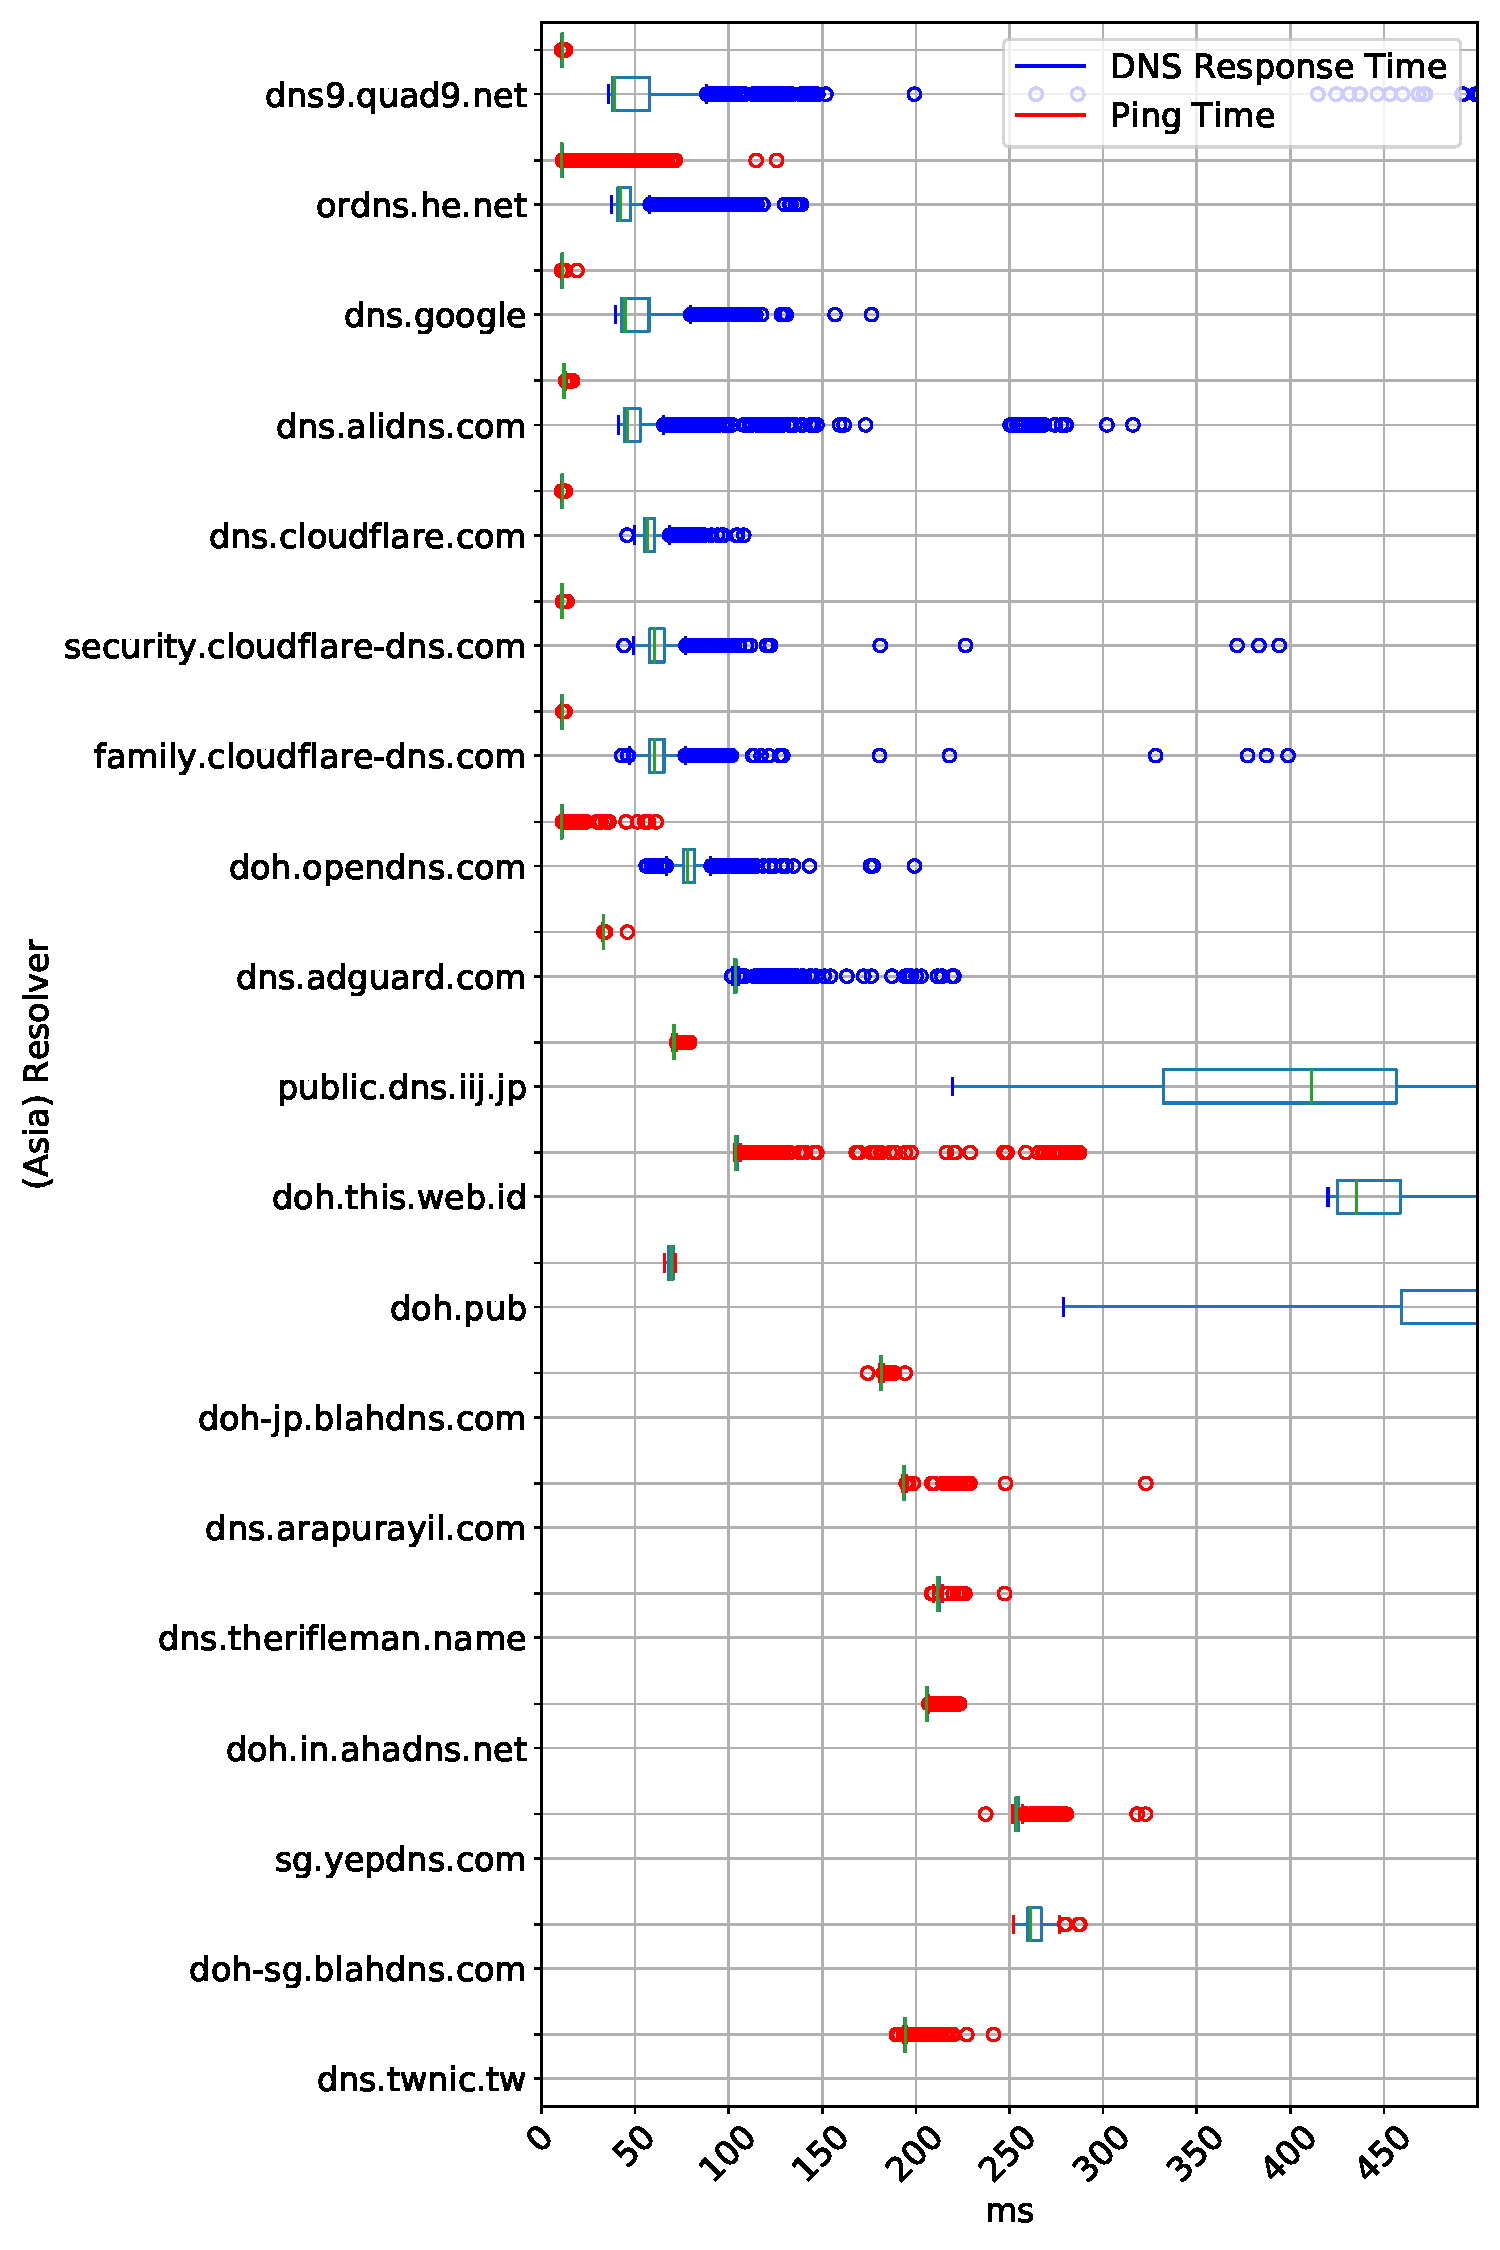
\includegraphics[width=0.32\linewidth]{figures/Ohio_Asia.pdf}}%
\hfill%
\subfigure[Europe.]{%
\label{fig:Ohio_Europe}%
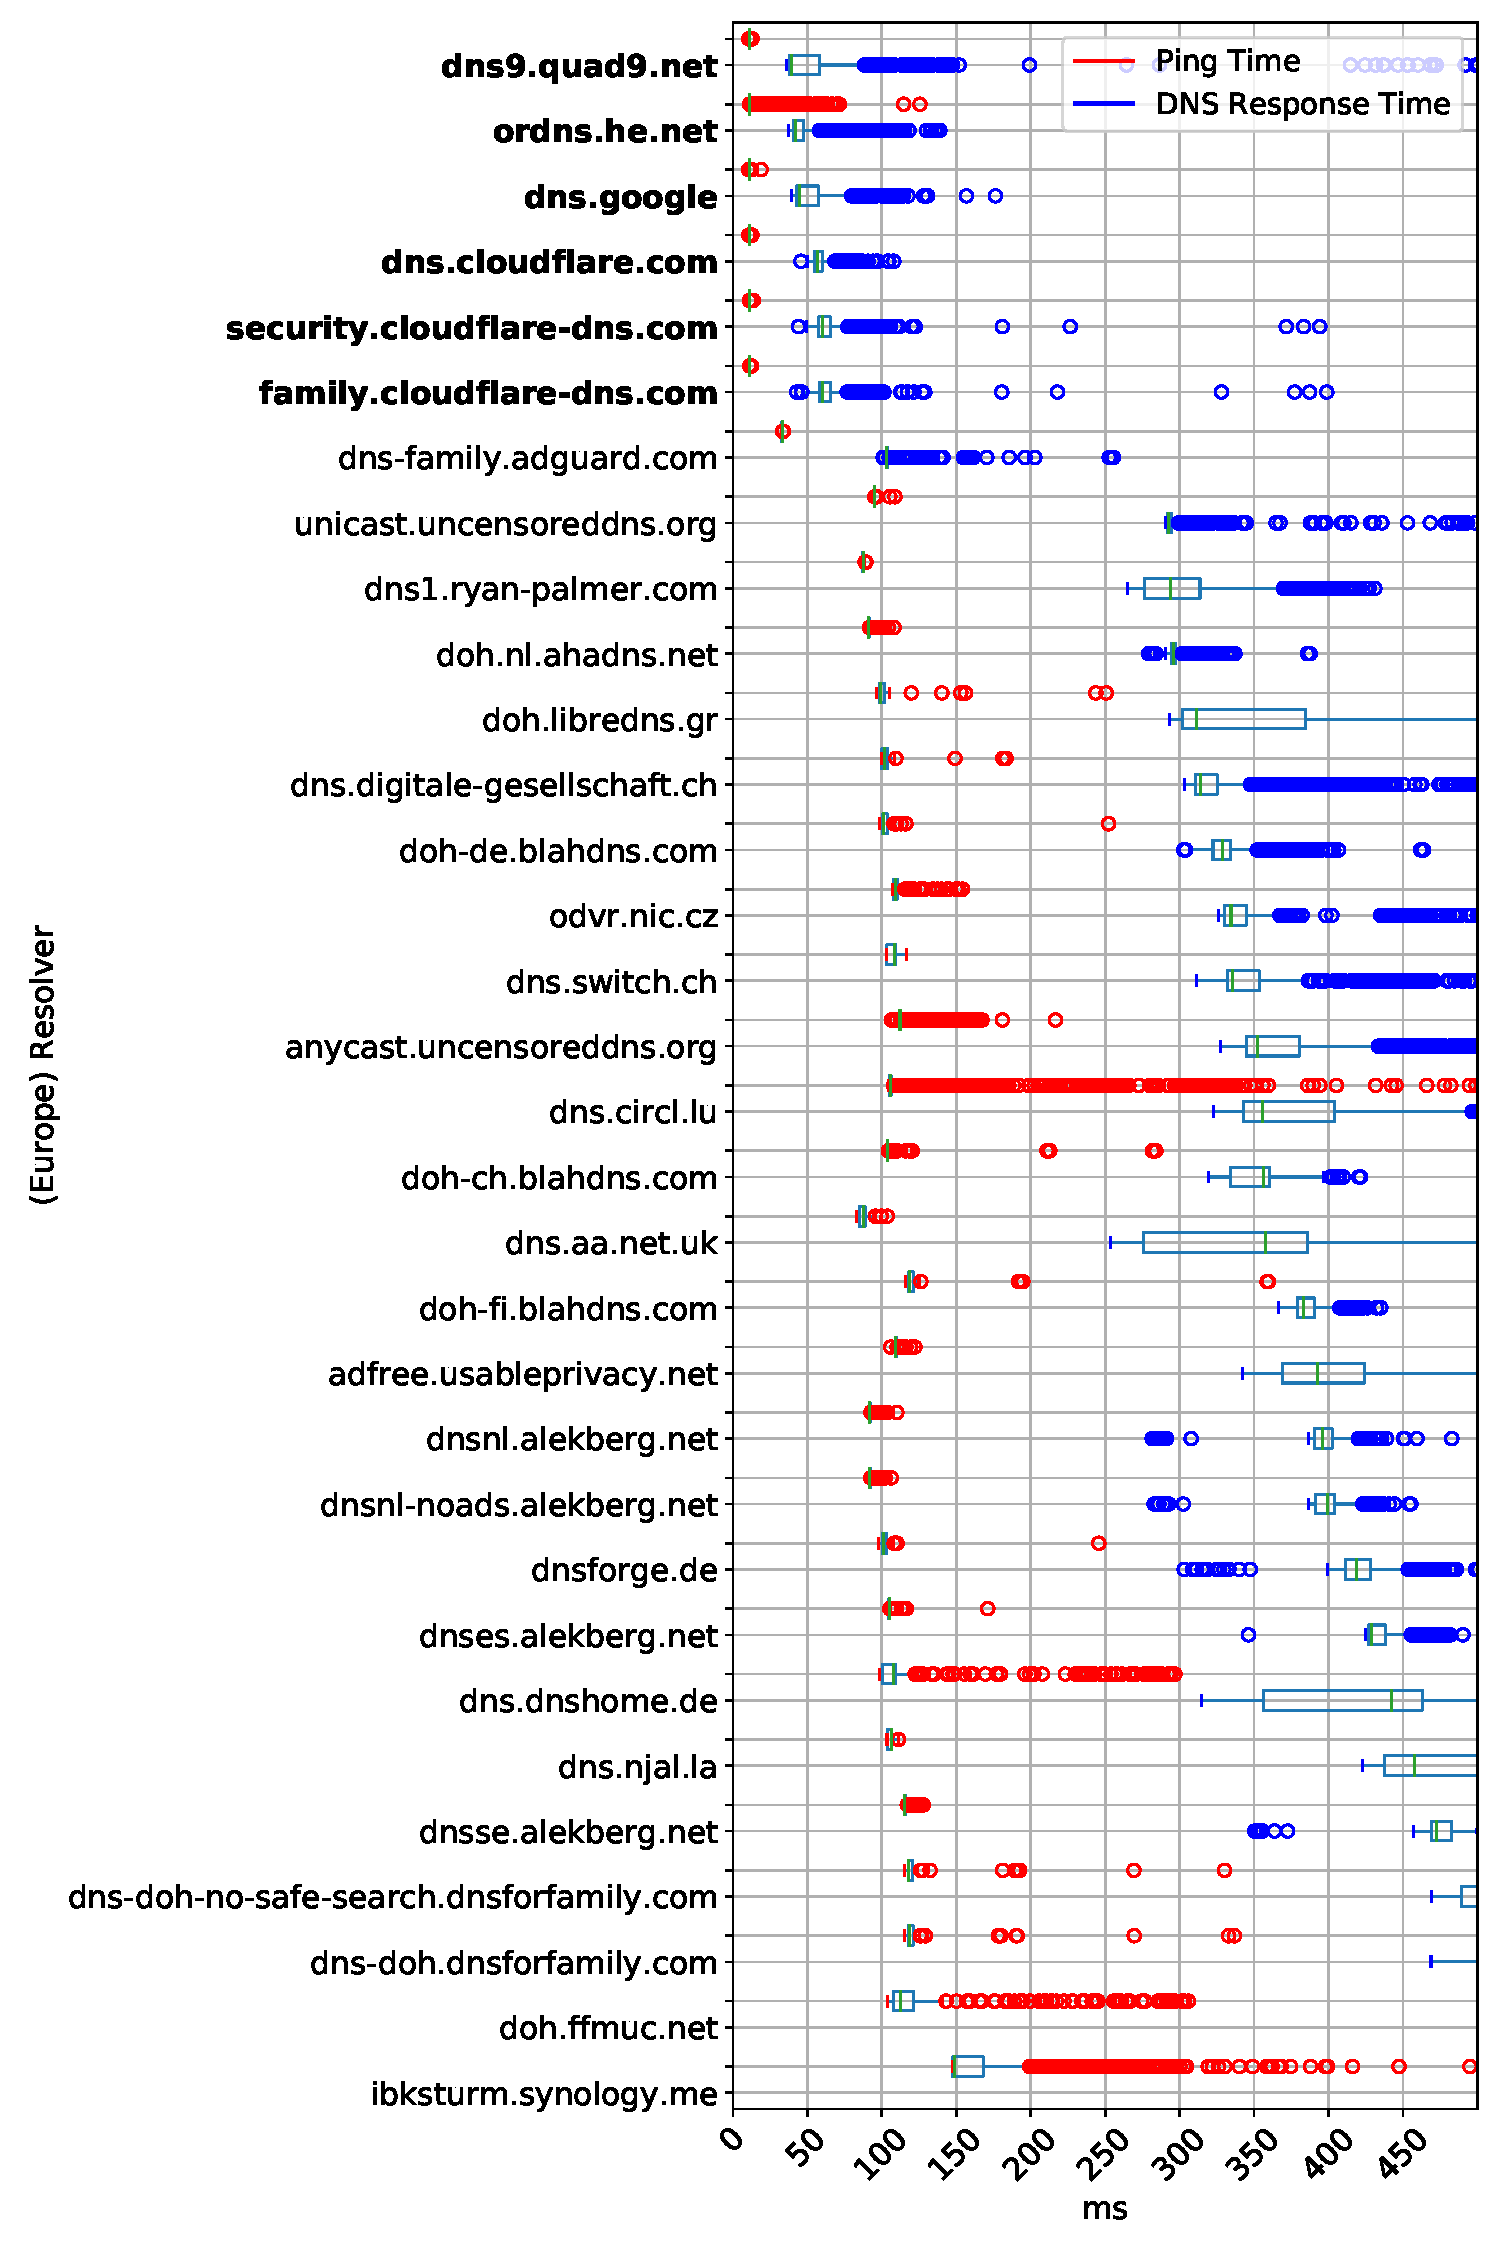
\includegraphics[width=0.32\linewidth]{figures/Ohio_Europe.pdf}}%
    \caption{Resolvers measured from a vantage point in the United States (Ohio).}
\end{minipage}
\end{figure}

\subsection{\mbox{How Do Non-Mainstream Resolvers Perform?}}

Given the large number of non-mainstream resolvers, we aimed to study how
the performance of these encrypted DNS resolvers to mainstream ones.
In most cases, as expected, mainstream resolvers outperformed non-mainstream resolvers.
Non-mainstream resolvers also exhibited higher variability of 
median query response times.  
From North America, we observe that aside from the top five resolvers,
median query response times ranged from \xxx{X}
ms to \xxx{X} ms.  From Asia, median response times outside
of the top five ranged from \xxx{X} ms to \xxx{X} ms.  We observe more
consistent performance from the Asia vantage point, but we still
see median query response times outside the top five range from \xxx{X} ms to
\xxx{X} ms.

In some cases, however, a particular non-mainstream resolver would outperform
the mainstream DoH resolvers.  As expected, \texttt{dns.quad9.net},
\texttt{dns.google}, and \texttt{dns.cloudflare.com} were among the top five
highest performing DoH resolvers in North America, Europe, and Asia.
Interestingly, however, \texttt{ordns.he.net}---a DoH resolver hosted by
Hurricane Electric, a global Internet service provider (ISP)---managed to
outperform \texttt{dns.google} and \texttt{dns.cloudflare.com} from all three
vantage points.  From Frankfurt, \texttt{dns-family.adguard.com} and
\texttt{ordns.he.net} are the top two highest performing resolvers; from
Seoul, \texttt{doh-jp.blahdns.com} outperforms \texttt{dns.google}.

\begin{figure}[t!]
\hspace*{-1in}
\begin{minipage}{1.35\textwidth}
\centering
\subfigure[North America.]{%
\label{fig:Seoul_NA}%
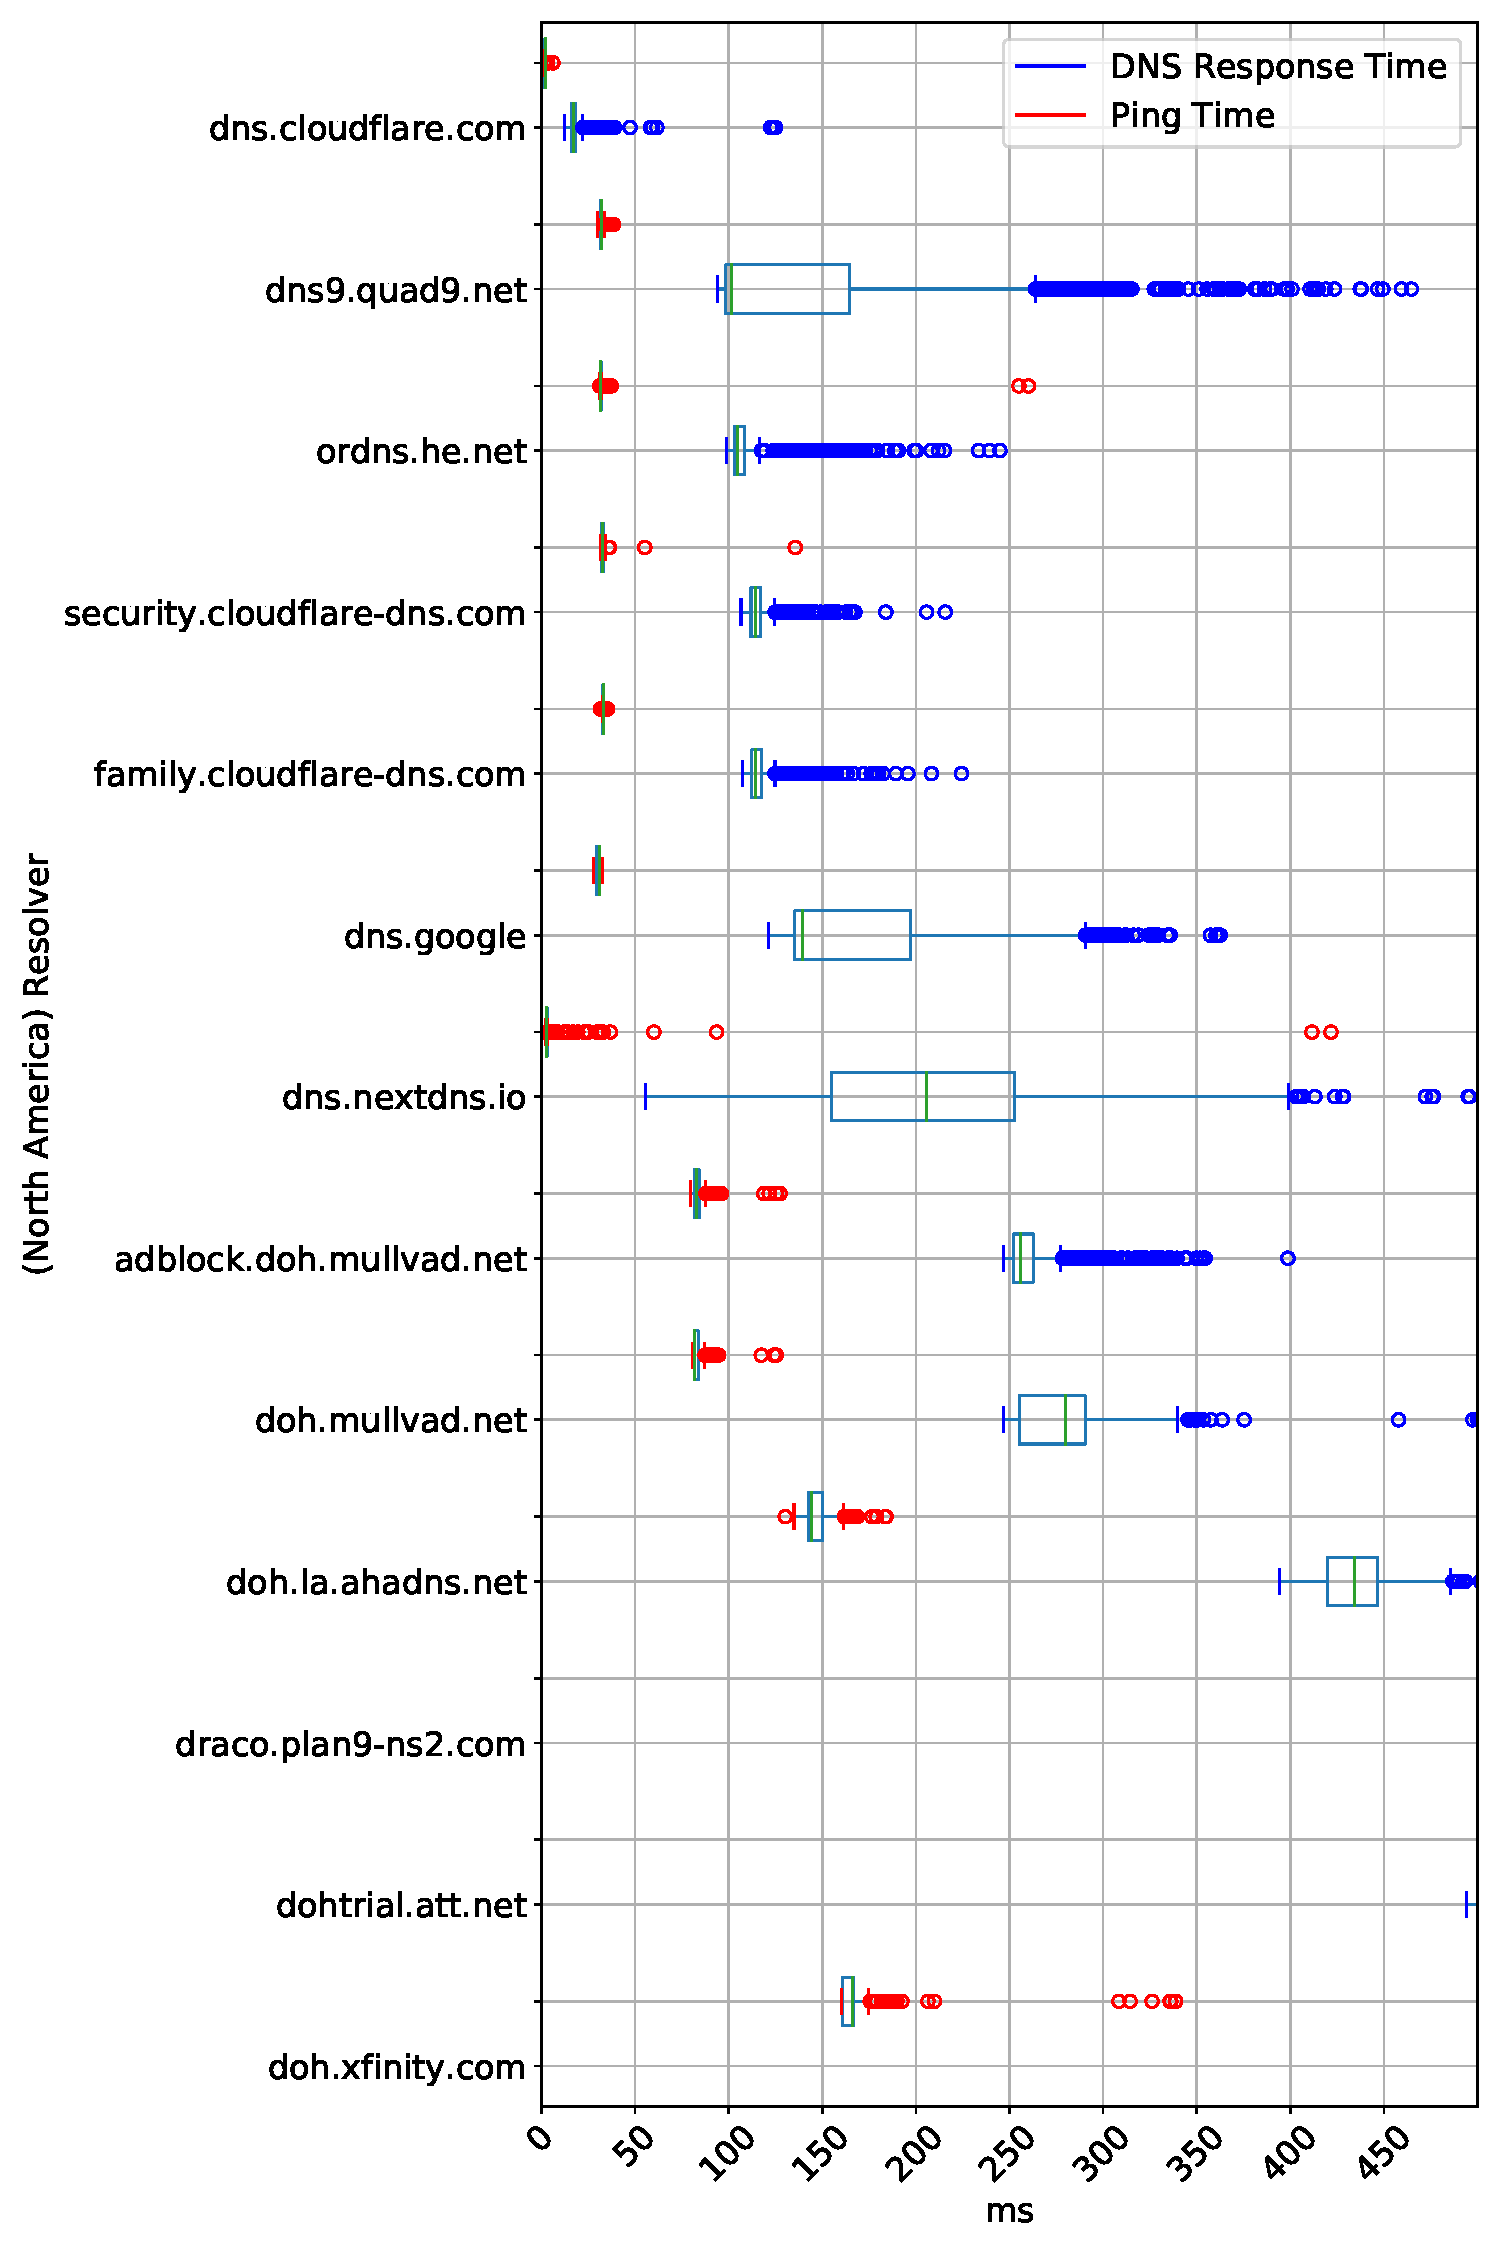
\includegraphics[width=0.32\linewidth]{figures/Seoul_North_America.pdf}}%
\hfill%
    \subfigure[Asia (Local).]{%
\label{fig:Seoul_Asia}%
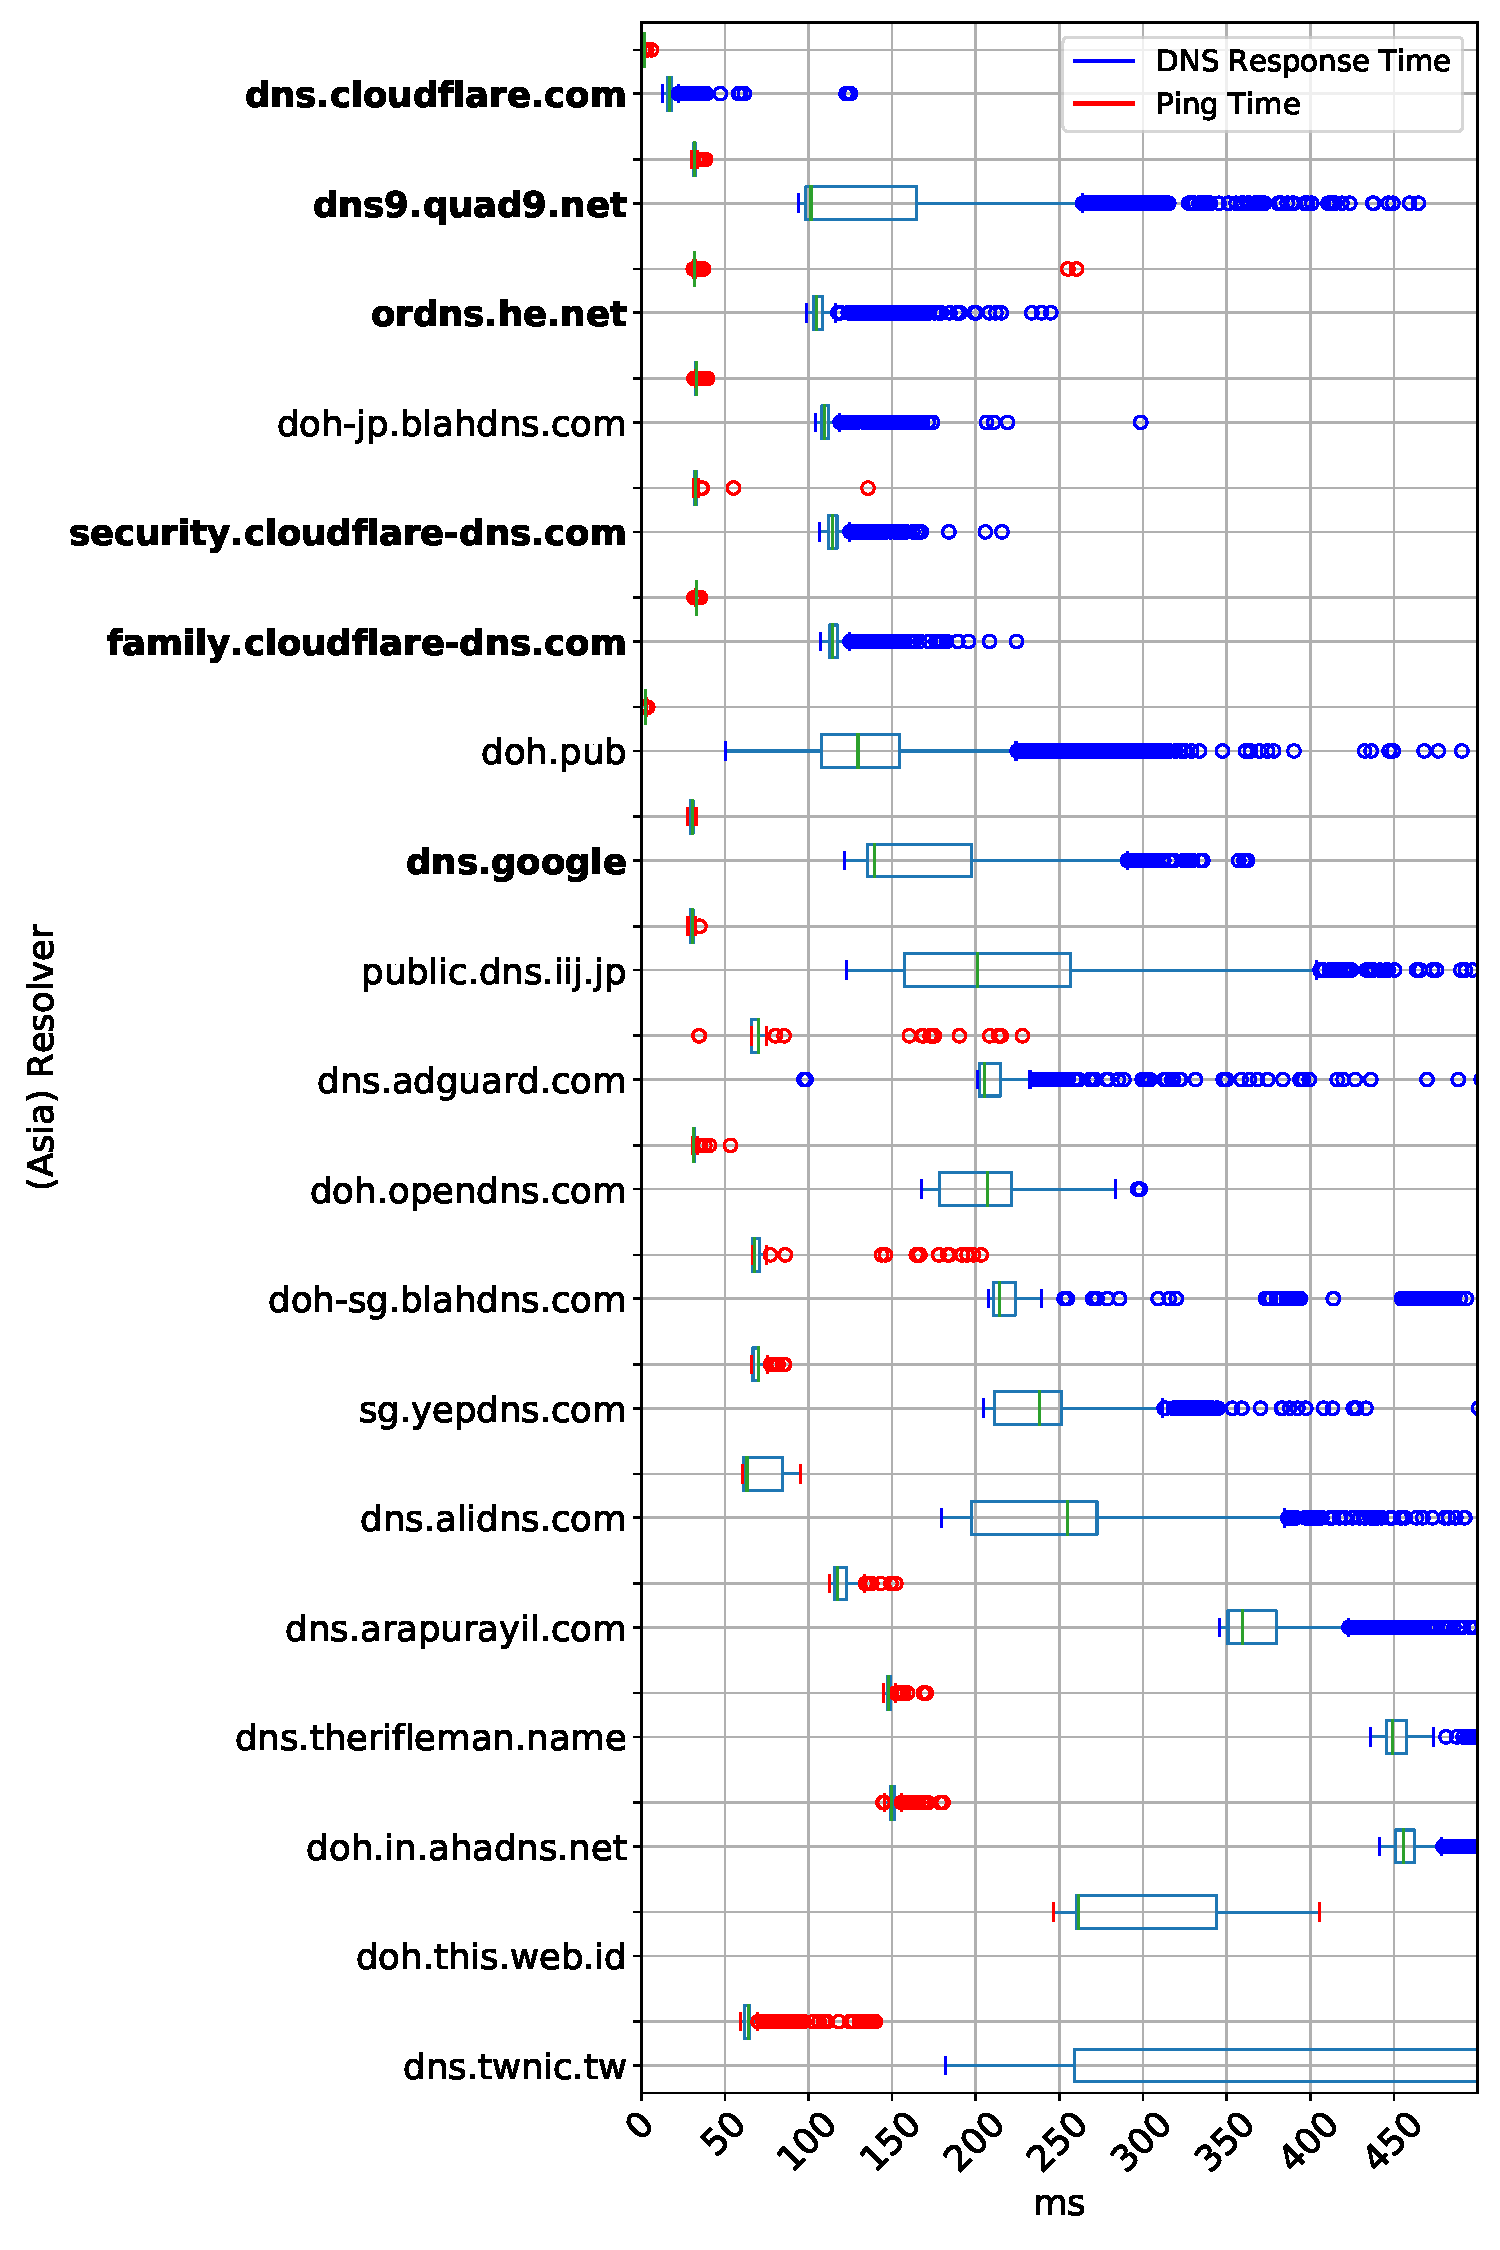
\includegraphics[width=0.32\linewidth]{figures/Seoul_Asia.pdf}}%
\hfill%
\subfigure[Europe.]{%
\label{fig:Seoul_Europe}%
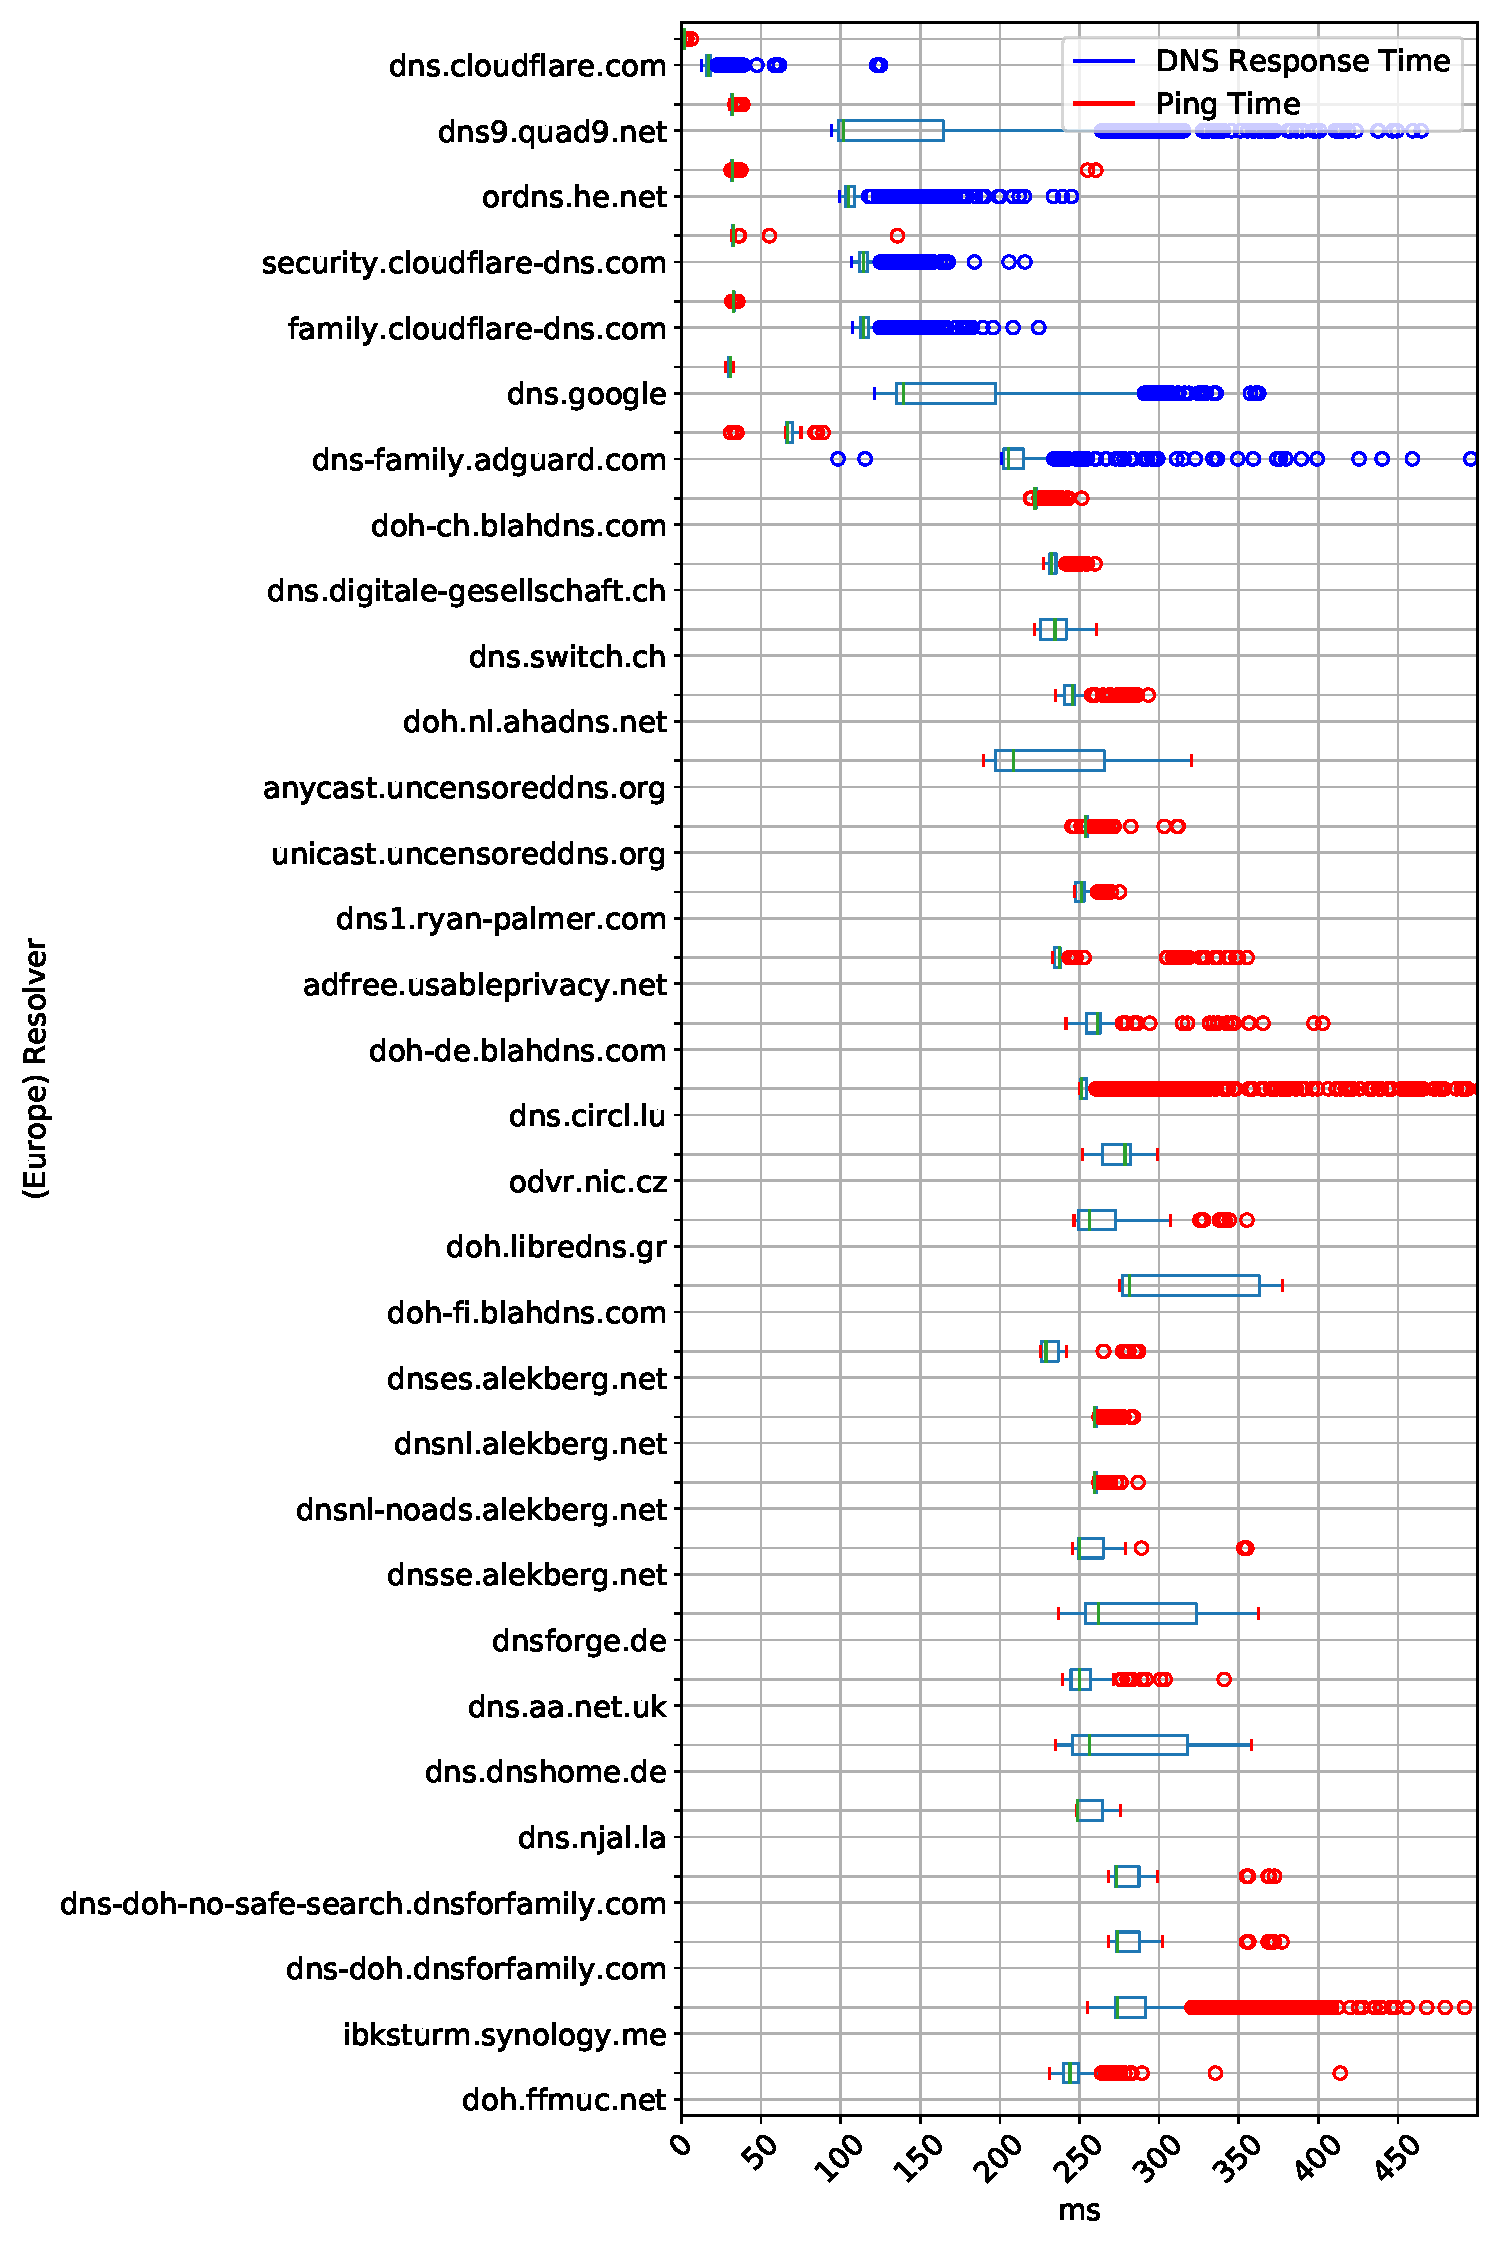
\includegraphics[width=0.32\linewidth]{figures/Seoul_Europe.pdf}}%
\caption{Resolvers measured from a vantage point in Seoul, South Korea.}
\end{minipage}
\end{figure}

\if 0
\begin{table}[t!]
\centering
\begin{tabular}{ll}
\hline
\textbf{Location} & \textbf{Resolver}                                                                               \\ \hline
North America     & ordns.he.net                                                                                    \\ \hline
Asia              & \begin{tabular}[c]{@{}l@{}}ordns.he.net\\ doh-jp.blahdns.com\end{tabular}                       \\ \hline
Europe            & \begin{tabular}[c]{@{}l@{}}ordns.he.net\\ dns-family.adguard.com\\ doh.libredns.gr\end{tabular} \\ \hline
\end{tabular}
\caption{Non-mainstream resolvers that outperformed mainstream resolvers.}
\label{tab:outperformed_resolvers}
\end{table}
\fi




\begin{figure}[t!]
\hspace*{-1in}
\begin{minipage}{1.35\textwidth}
\centering
\subfigure[North America.]{%
\label{fig:Frankfurt_NA}%
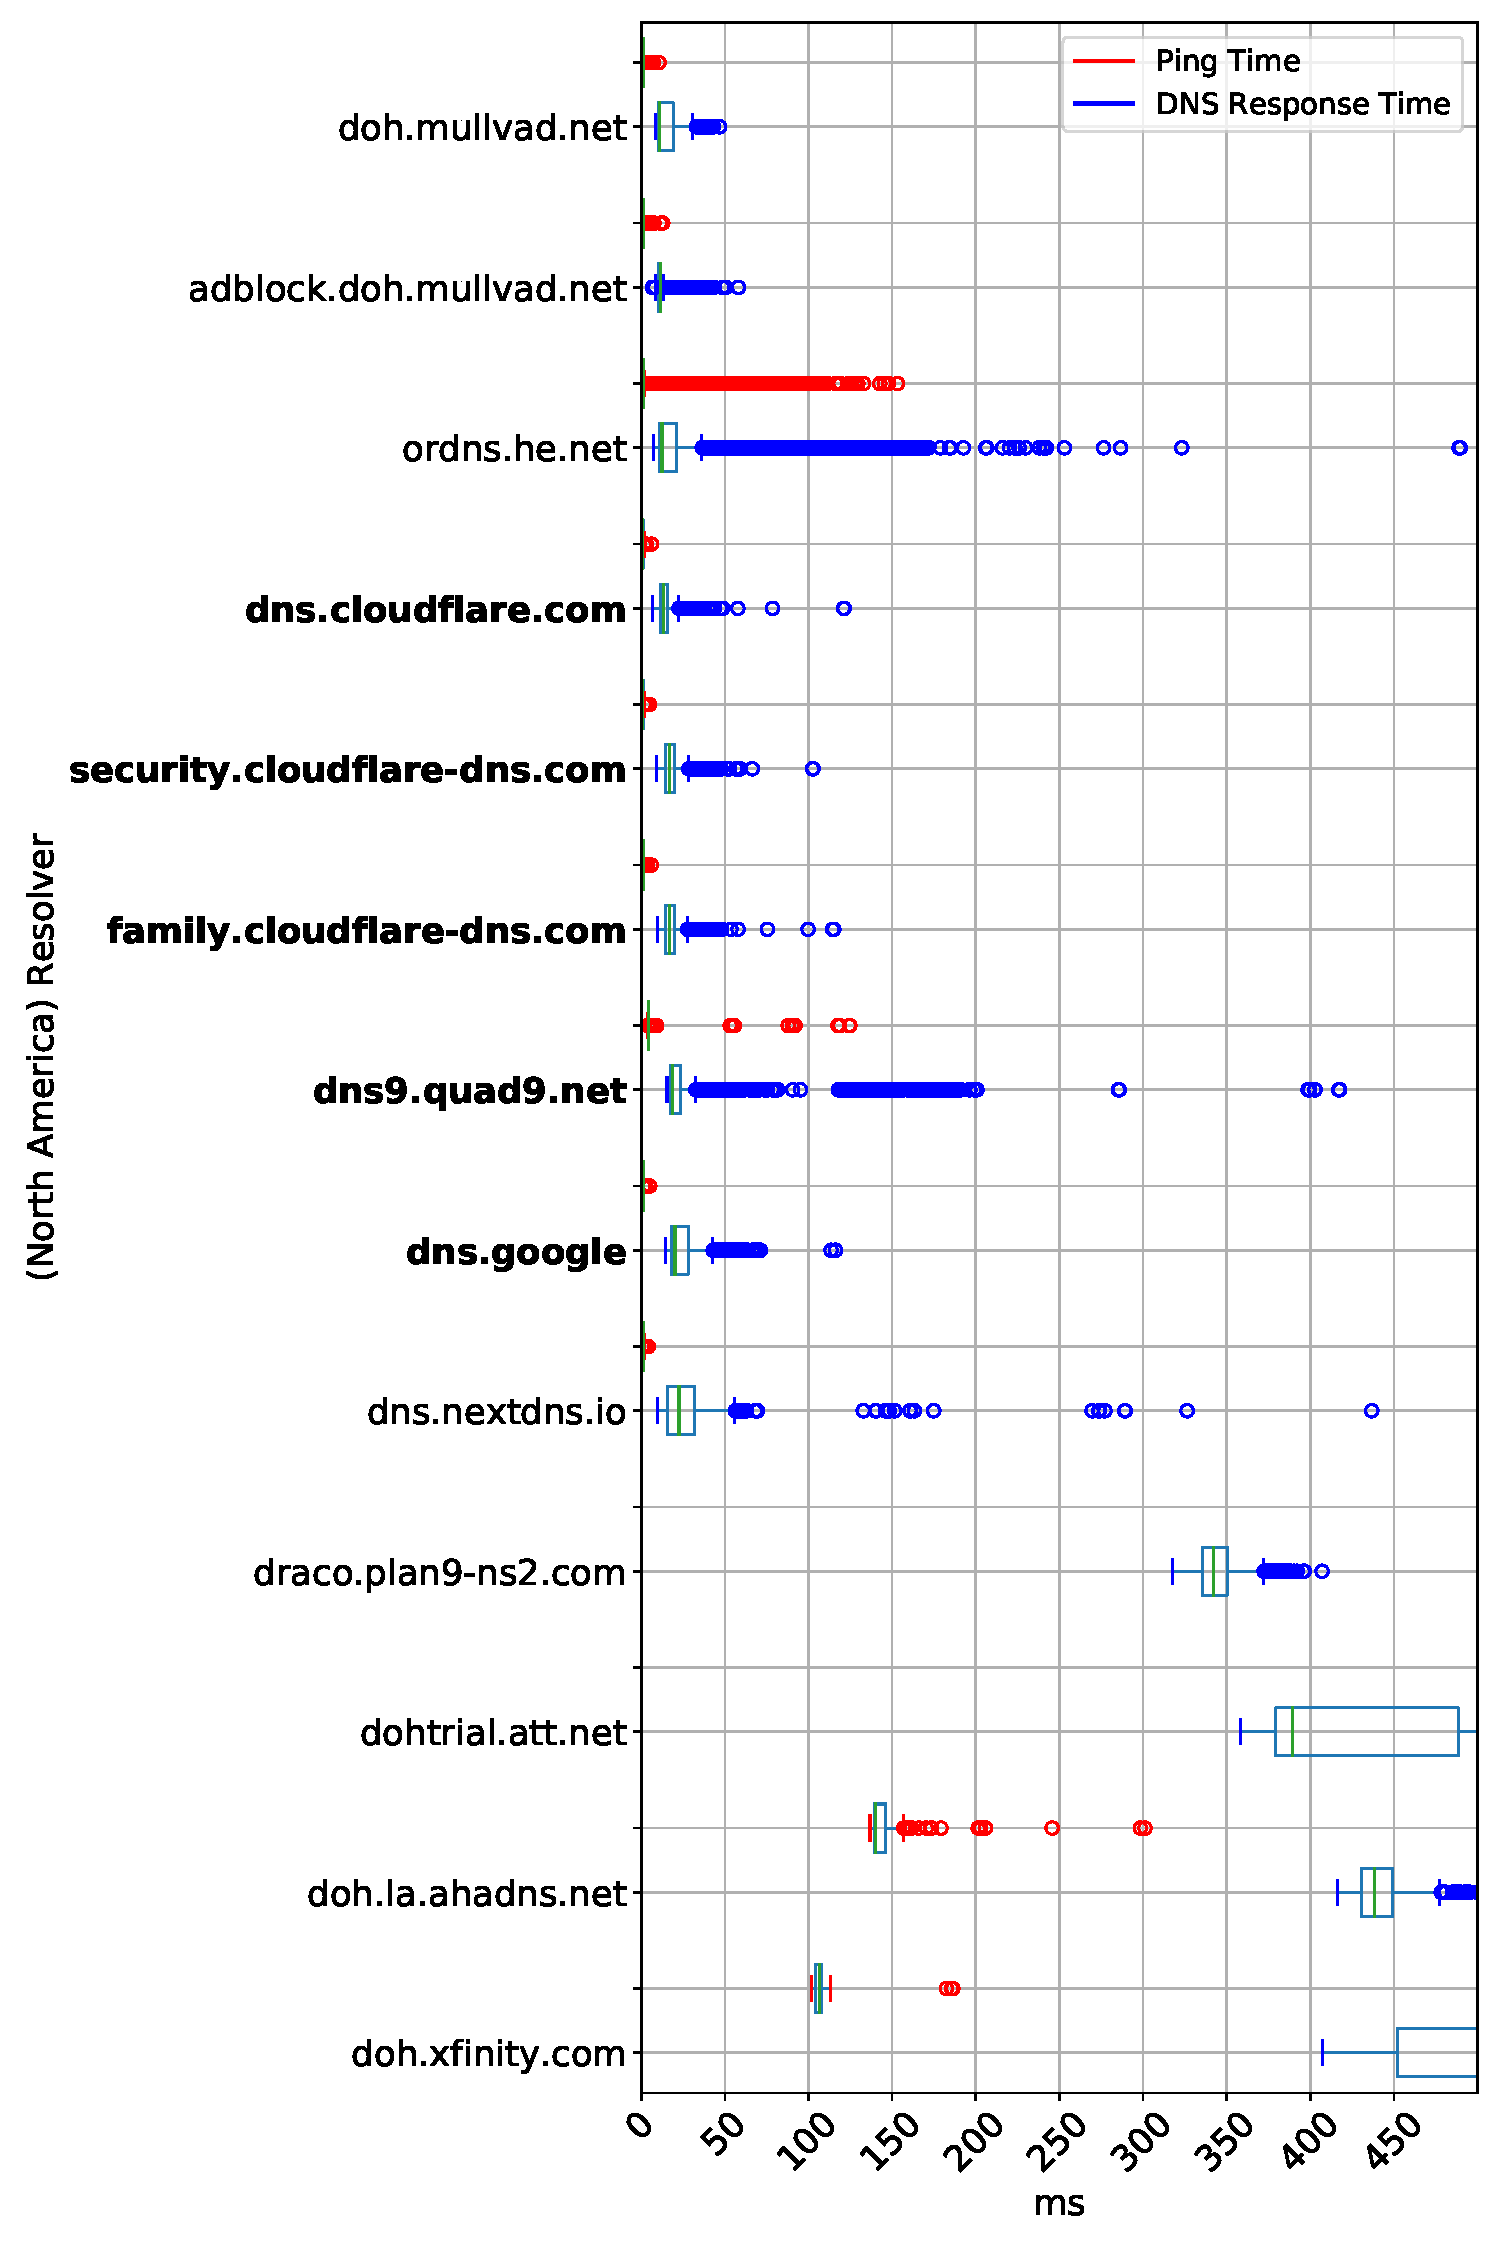
\includegraphics[width=0.32\linewidth]{figures/Frankfurt_North_America.pdf}}%
\hfill%
\subfigure[Asia. ]{%
\label{fig:Frankfurt_Asia}%
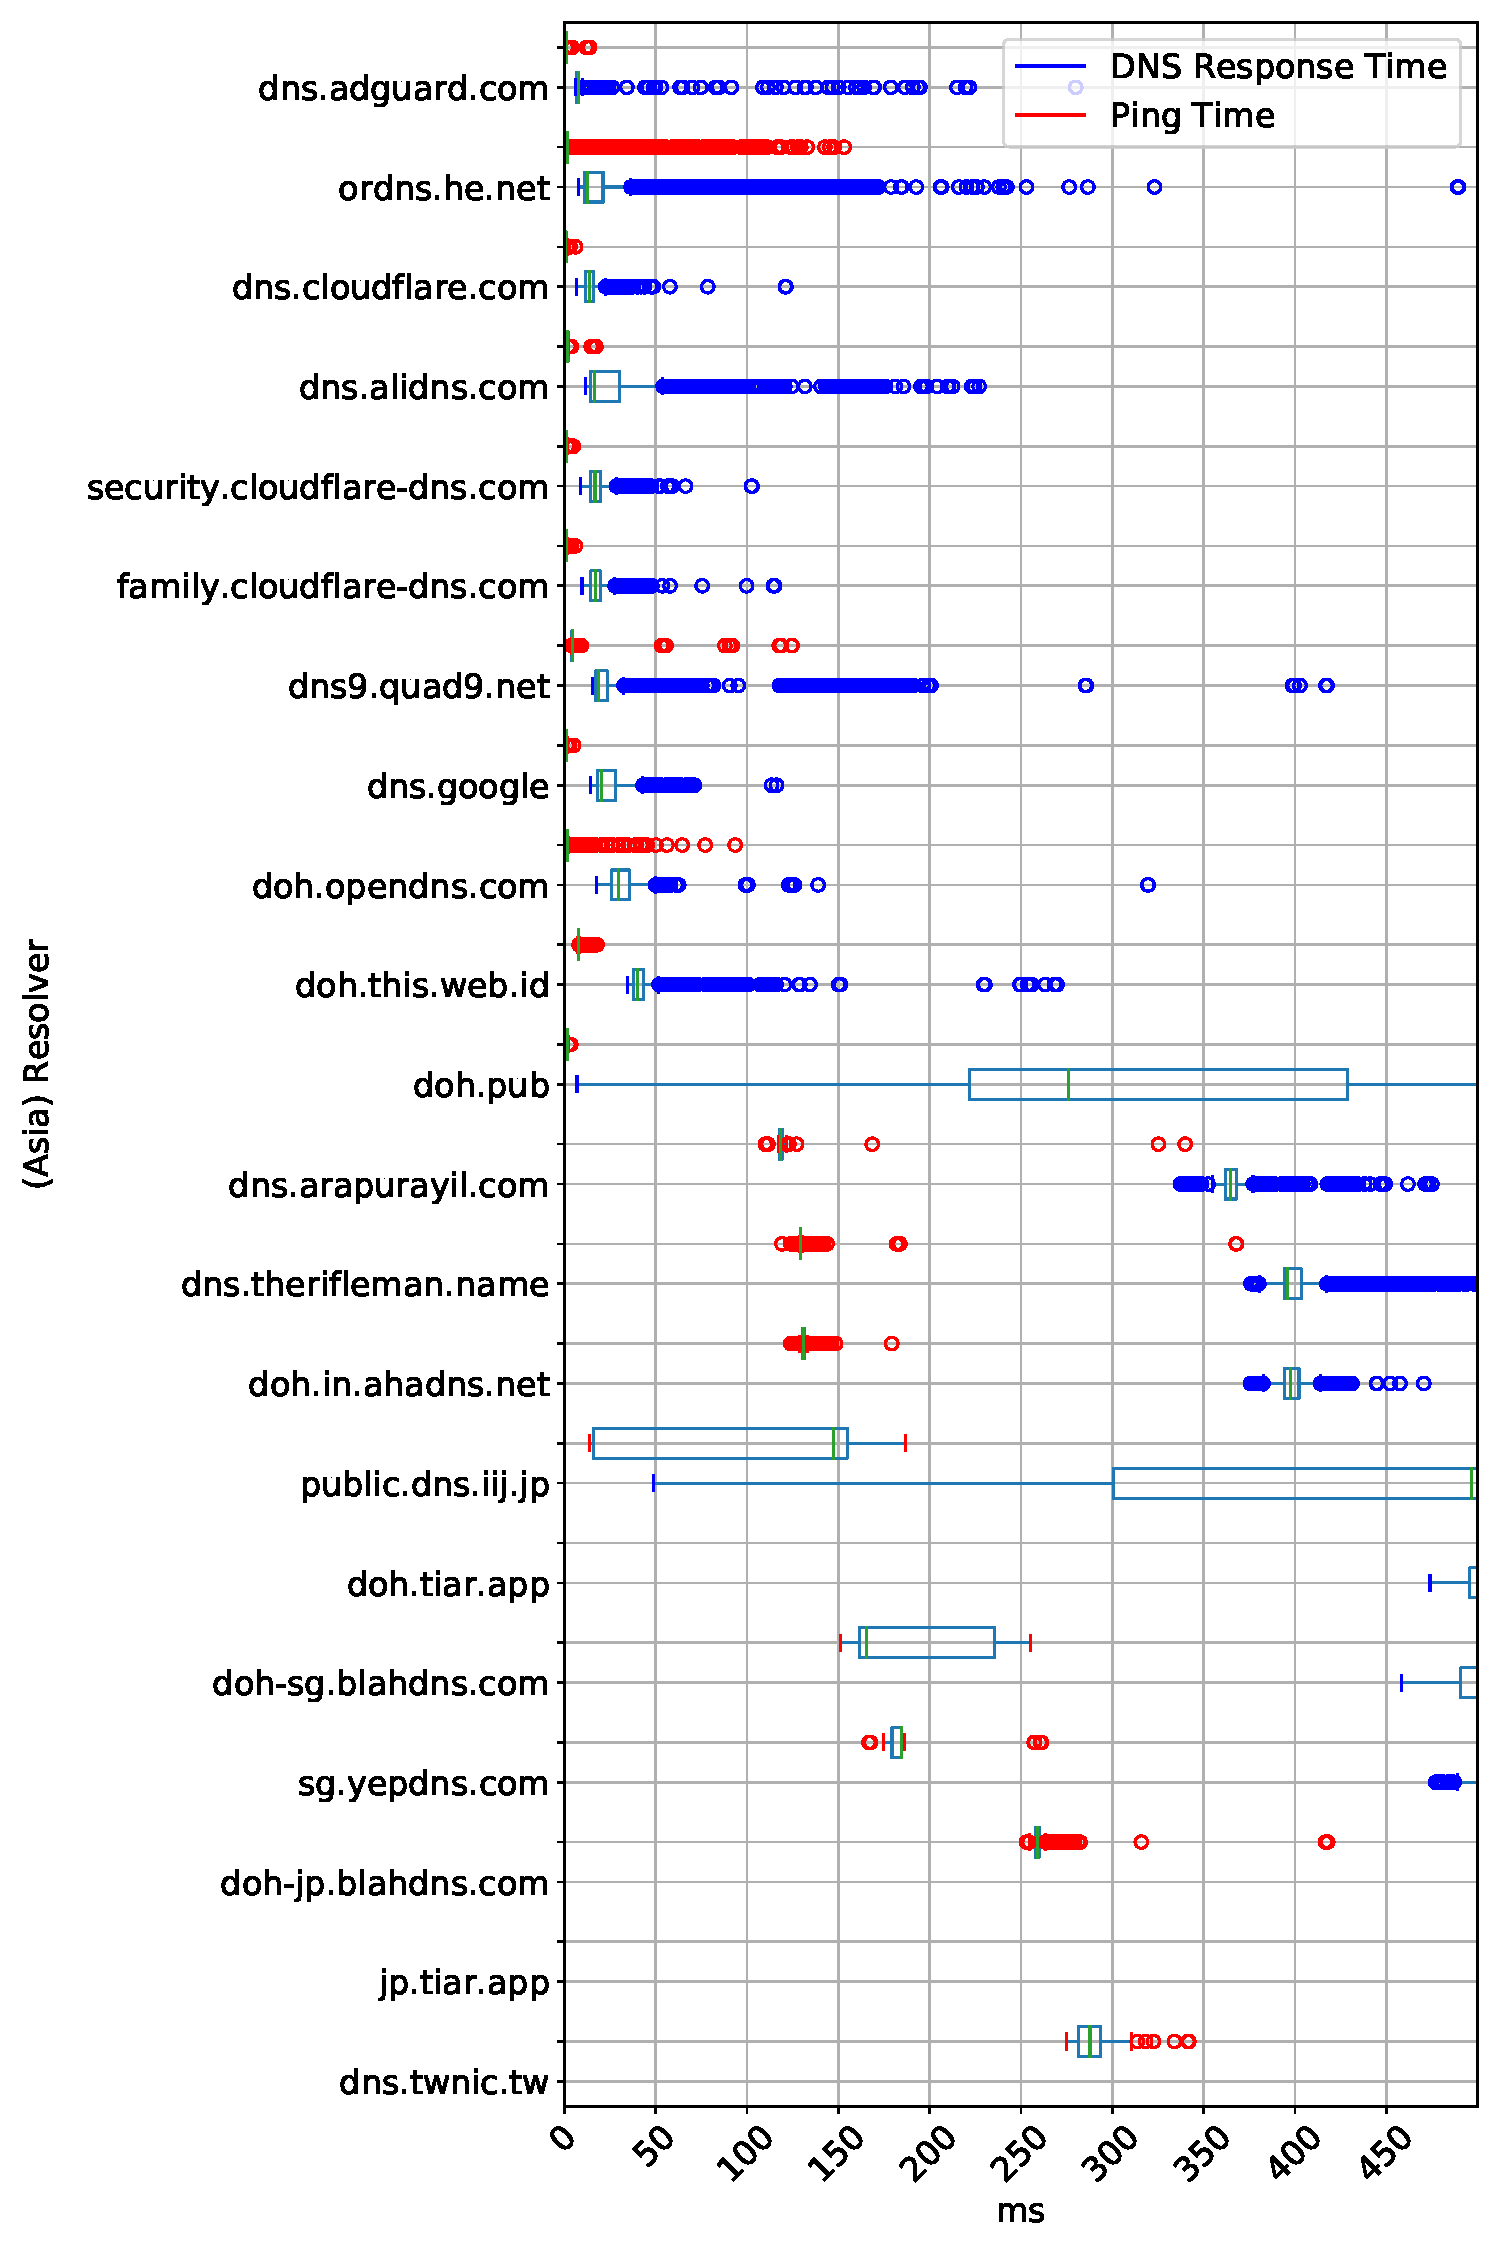
\includegraphics[width=0.32\linewidth]{figures/Frankfurt_Asia.pdf}}%
\hfill%
\subfigure[Europe (Local).]{%
\label{fig:Frankfurt_Europe}%
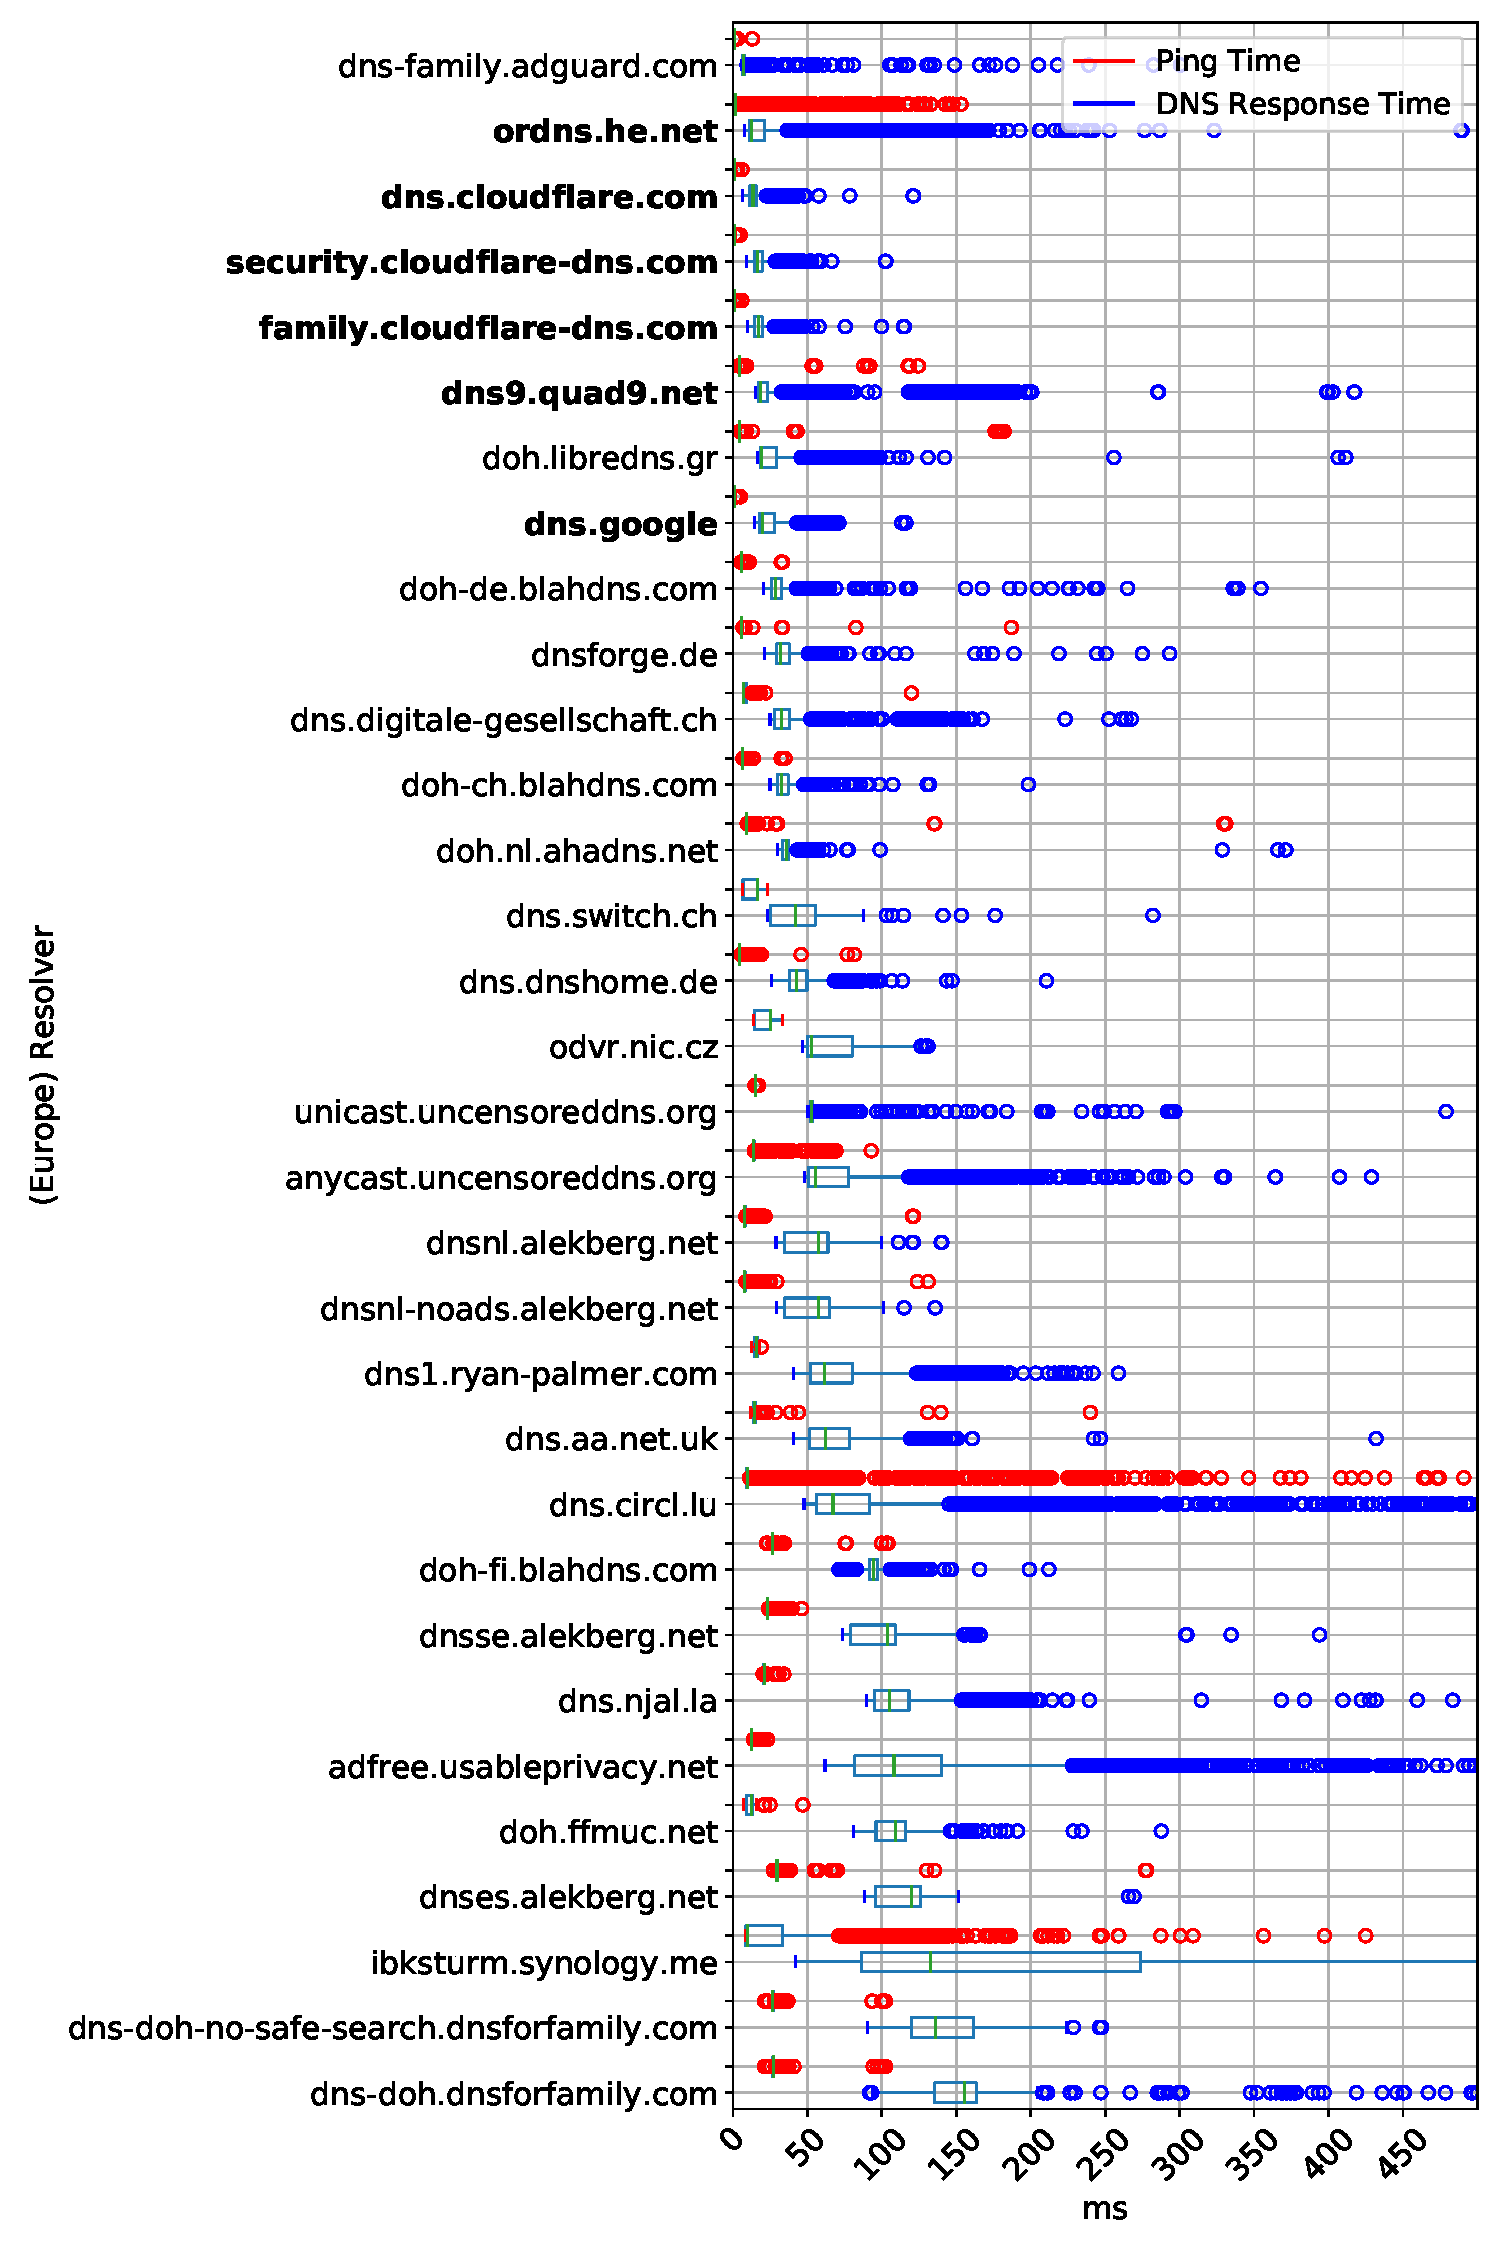
\includegraphics[width=0.32\linewidth]{figures/Frankfurt_Europe.pdf}}%
\caption{Resolvers measured from a vantage point in Frankfurt, Germany.}
\end{minipage}
\end{figure}

\subsection{Does Latency to Resolver Correlate with Performance?}
\begin{table}[t!]
\centering
\begin{tabular}{l|rr}
\toprule
    \textbf{Resolver} & \multicolumn{2}{c}{\textbf{Vantage Point}} \\
                  & \textrm{Seoul (ms)}         & \textrm{Frankfurt (ms)} \\
\midrule
dns.twnic.tw                                & 326.19 & 32,374.03                            \\
doh-jp.blahdns.com                          & 109.41                                           & 754.26                              \\
sg.yepdns.com                               & 232.69                                           & 540.19                              \\
public.dns.iij.jp                           & 206.37                                           & 506.05                              \\
doh-sg.blahdns                              & 221.41                                           & 498.76                              \\
\bottomrule
\end{tabular}
\caption{Median DNS response times for non-conventional resolvers located in Asia.}
\label{tab:UnconvAsia}
\end{table}

\begin{table}[t!]
\centering
\begin{tabular}{l|rr}
\toprule
\textbf{Resolver} & \multicolumn{2}{c}{\textbf{Vantage Point}} \\
                  & \textrm{Frankfurt (ms)}     & \textrm{Seoul (ms)} \\
\midrule
doh.ffmuc.net                               & 109.15 & 1,307.21                         \\
ibksturm.synology.me                        & 85.77 & 1,227.35                         \\
dns-doh-no-safe-search.dnsforfamily         & 125.74 & 1,150.63                         \\
dnsforge.de                                 & 32.17 & 1,029.92                         \\
dns-doh.dnsforfamily                        & 153.74 & 1,153.29                         \\
\bottomrule
\end{tabular}
\caption{Median DNS response times for non-conventional resolvers located in Europe.}
\label{tab:UnconvEur}
\end{table}

We find that network distance correlates to higher encrypted DNS response
times.  Table~\ref{tab:UnconvAsia} shows that non-mainstream resolvers located
in Asia perform better from the vantage point in Seoul than the one in
Frankfurt.  Similarly, as expected, Table~\ref{tab:UnconvEur} shows that the
response times of non-mainstream resolvers in Europe are much lower when
measured from Frankfurt than the response times of those same resolvers
measured from Seoul.

Although higher network latency would tend to translate to higher DNS response
times (as encrypted DNS queries do require several network round rips), we
also found that, in some cases, certain resolvers performed worse than might
be expected as a result of the latency from the vantage point to the
resolvers.  For example, although the average round-trip latency to
\texttt{doh.in.ahadns.net} from our Seoul vantage point was \xxx{X} ms, the
median query response time was \xxx{X} ms.  Similarly, from North America, we
observed an average round-trip latency to \texttt{doh.xfinity.com} of
\texttt{X} ms, despite a median query response time of \xxx{X} ms.  We believe
this could be attributed these non-mainstream resolvers having especially
smaller caches than mainstream resolvers.  These discrepancies between network
latency and DNS response times may be due to a number of factors, including
both caching and server load. \AH{Review
this previous hypothesis later} We note that certain resolvers did not respond
to our ICMP ping messages (\Fref{tab:unresponsive}).


\if 0
\begin{figure}[t!]
\hspace*{-0.75in}
\begin{minipage}{1.25\textwidth}
\centering
\subfigure[North American resolvers measured from Ohio, USA]{%
\label{fig:Local_Ohio_NA}%
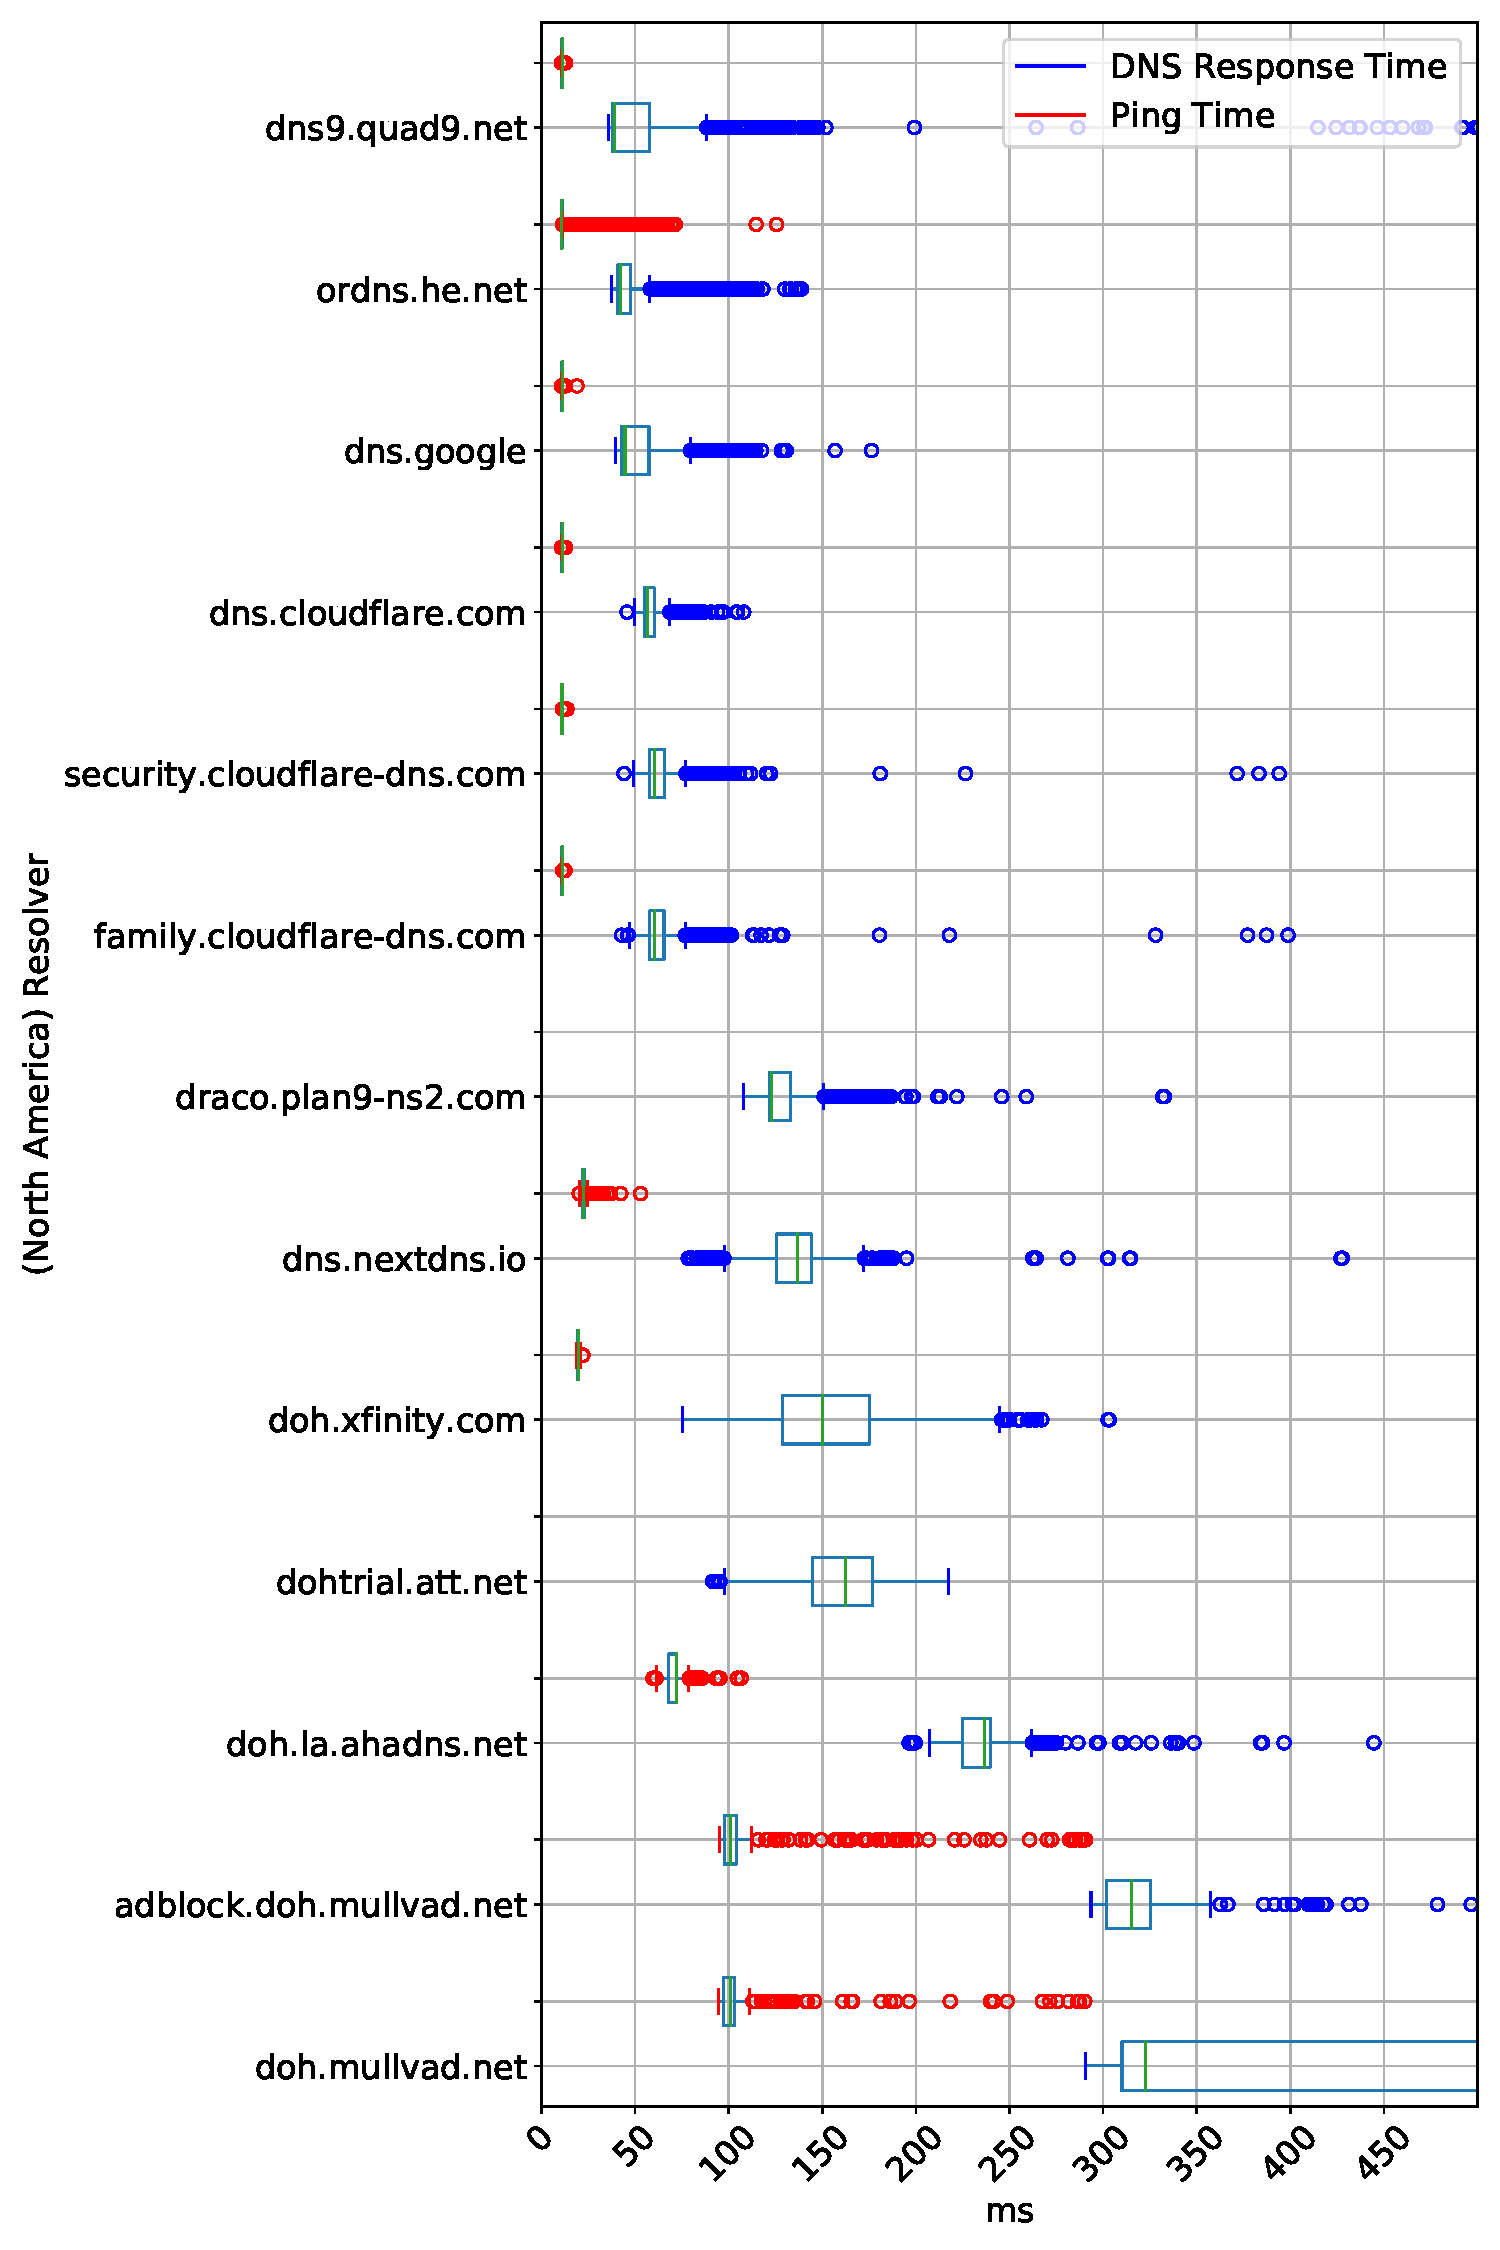
\includegraphics[width=0.32\linewidth]{figures/Ohio_North_America.pdf}}%
\hfill%
\subfigure[Asian resolvers measured from Seoul, South Korea]{%
\label{fig:Local_Seoul_Asia}%
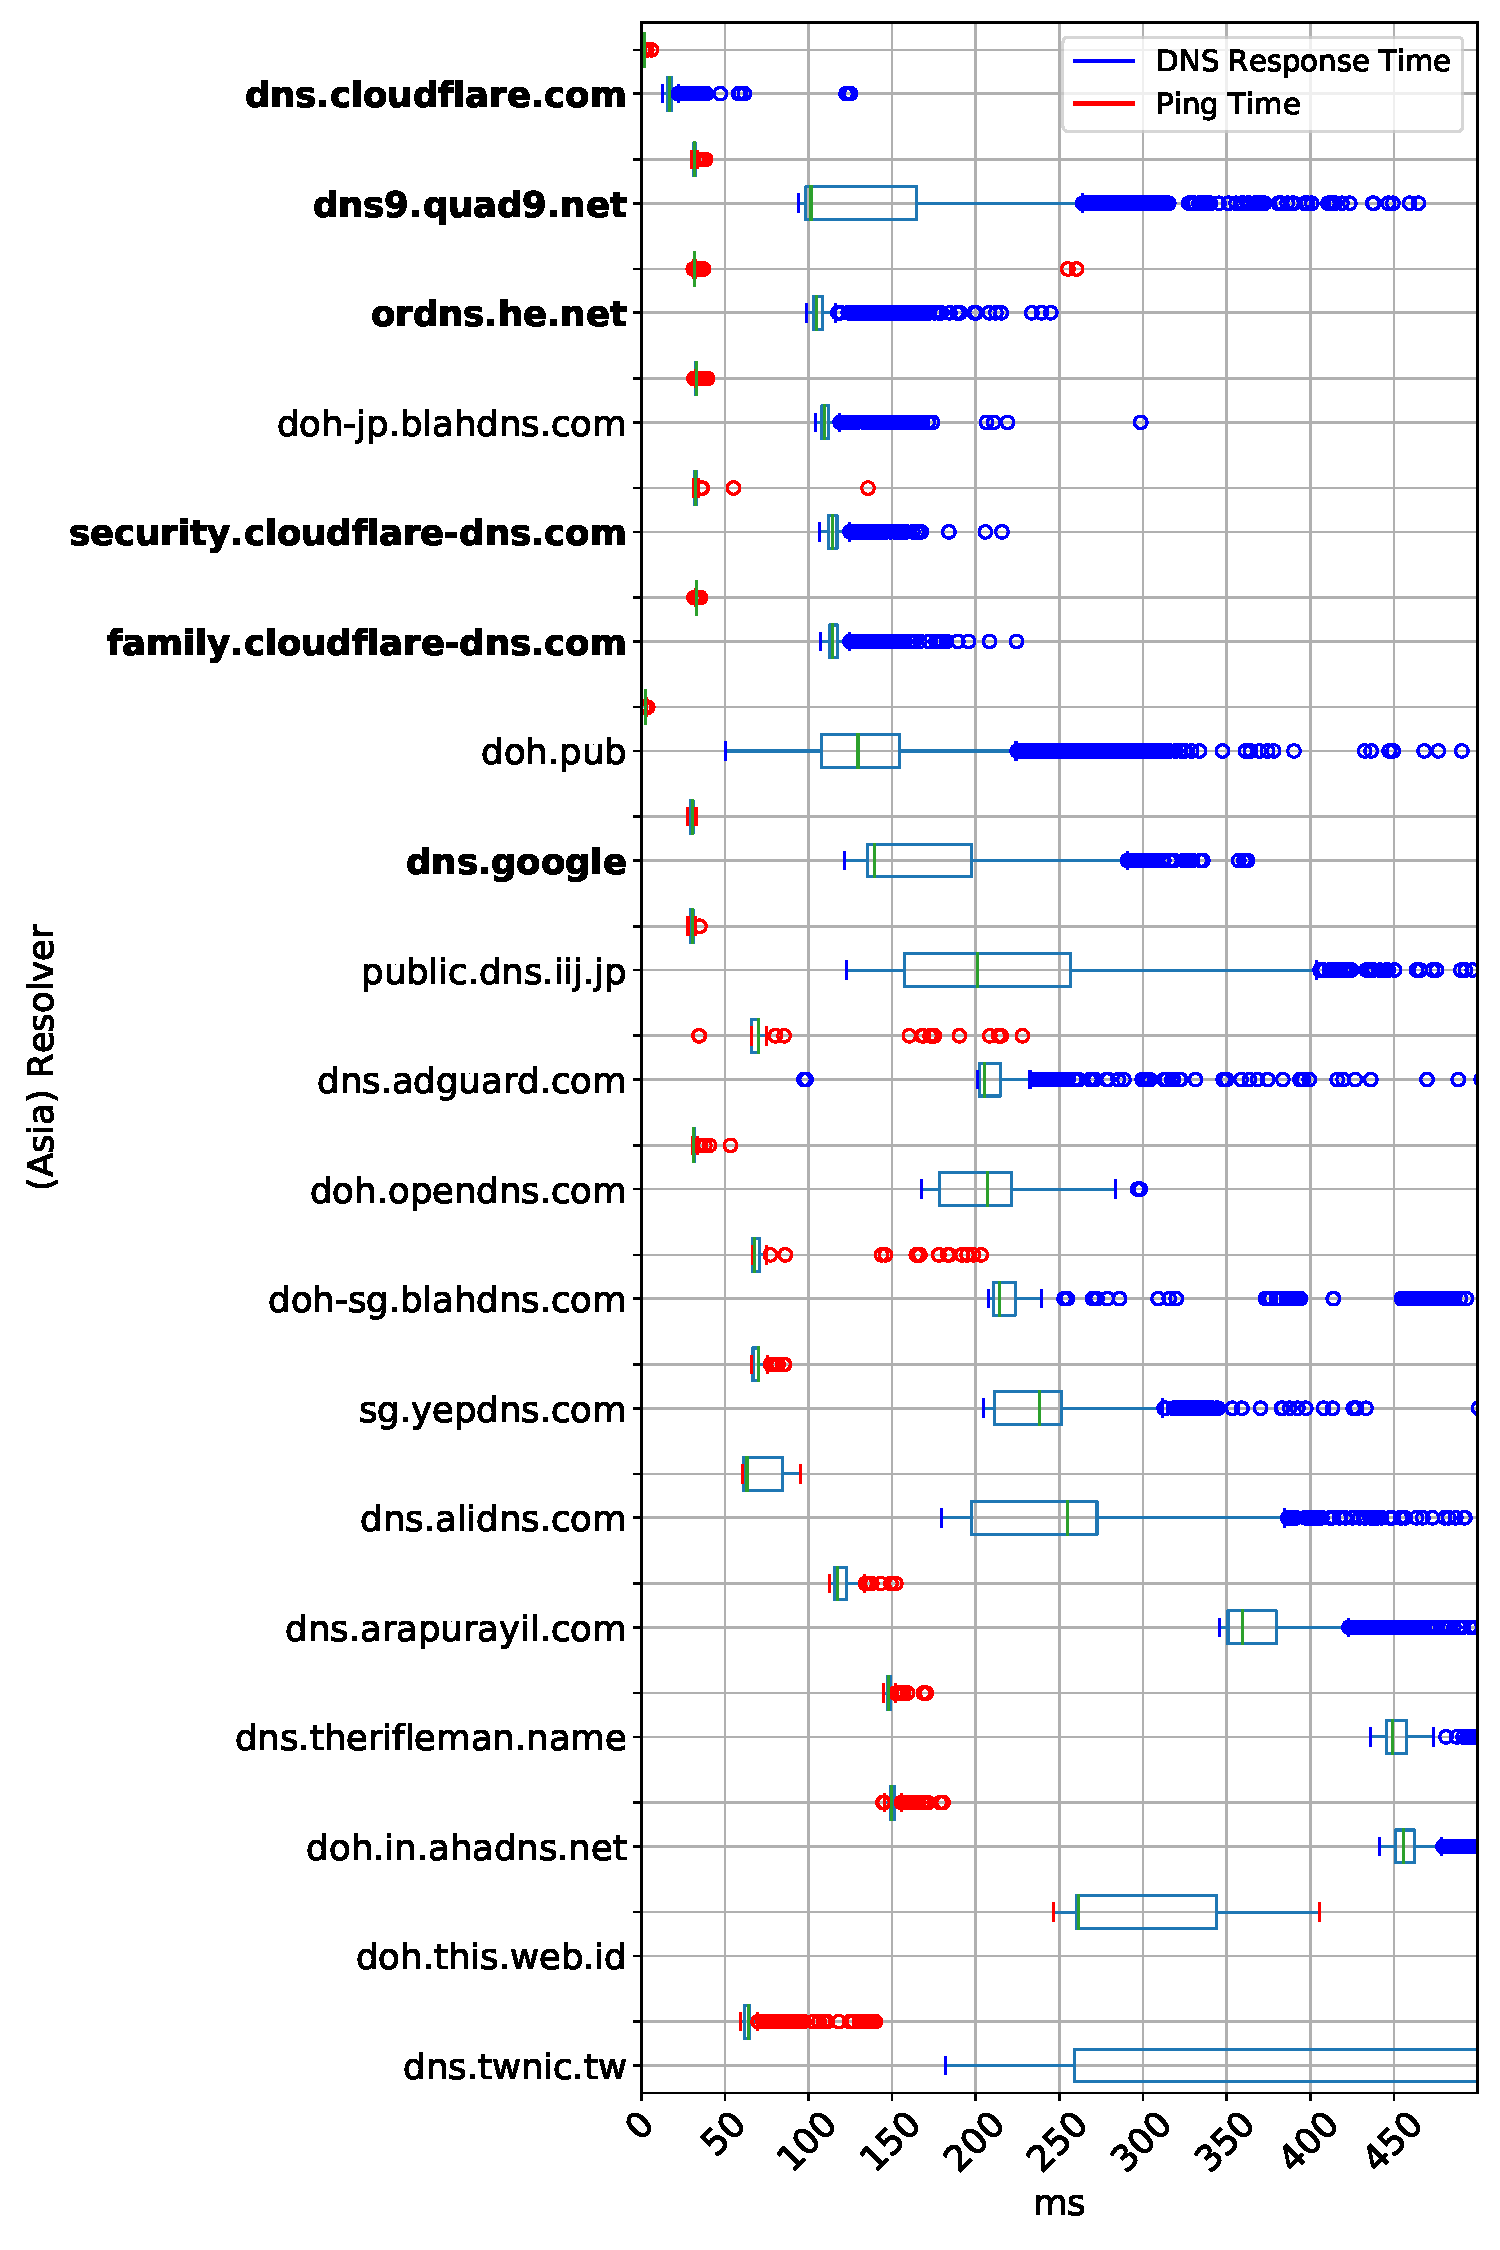
\includegraphics[width=0.32\linewidth]{figures/Seoul_Asia.pdf}}%
\hfill%
\subfigure[European resolvers measured from Frankfurt, Germany]{%
\label{fig:Kocal_Frankfurt_Europe}%
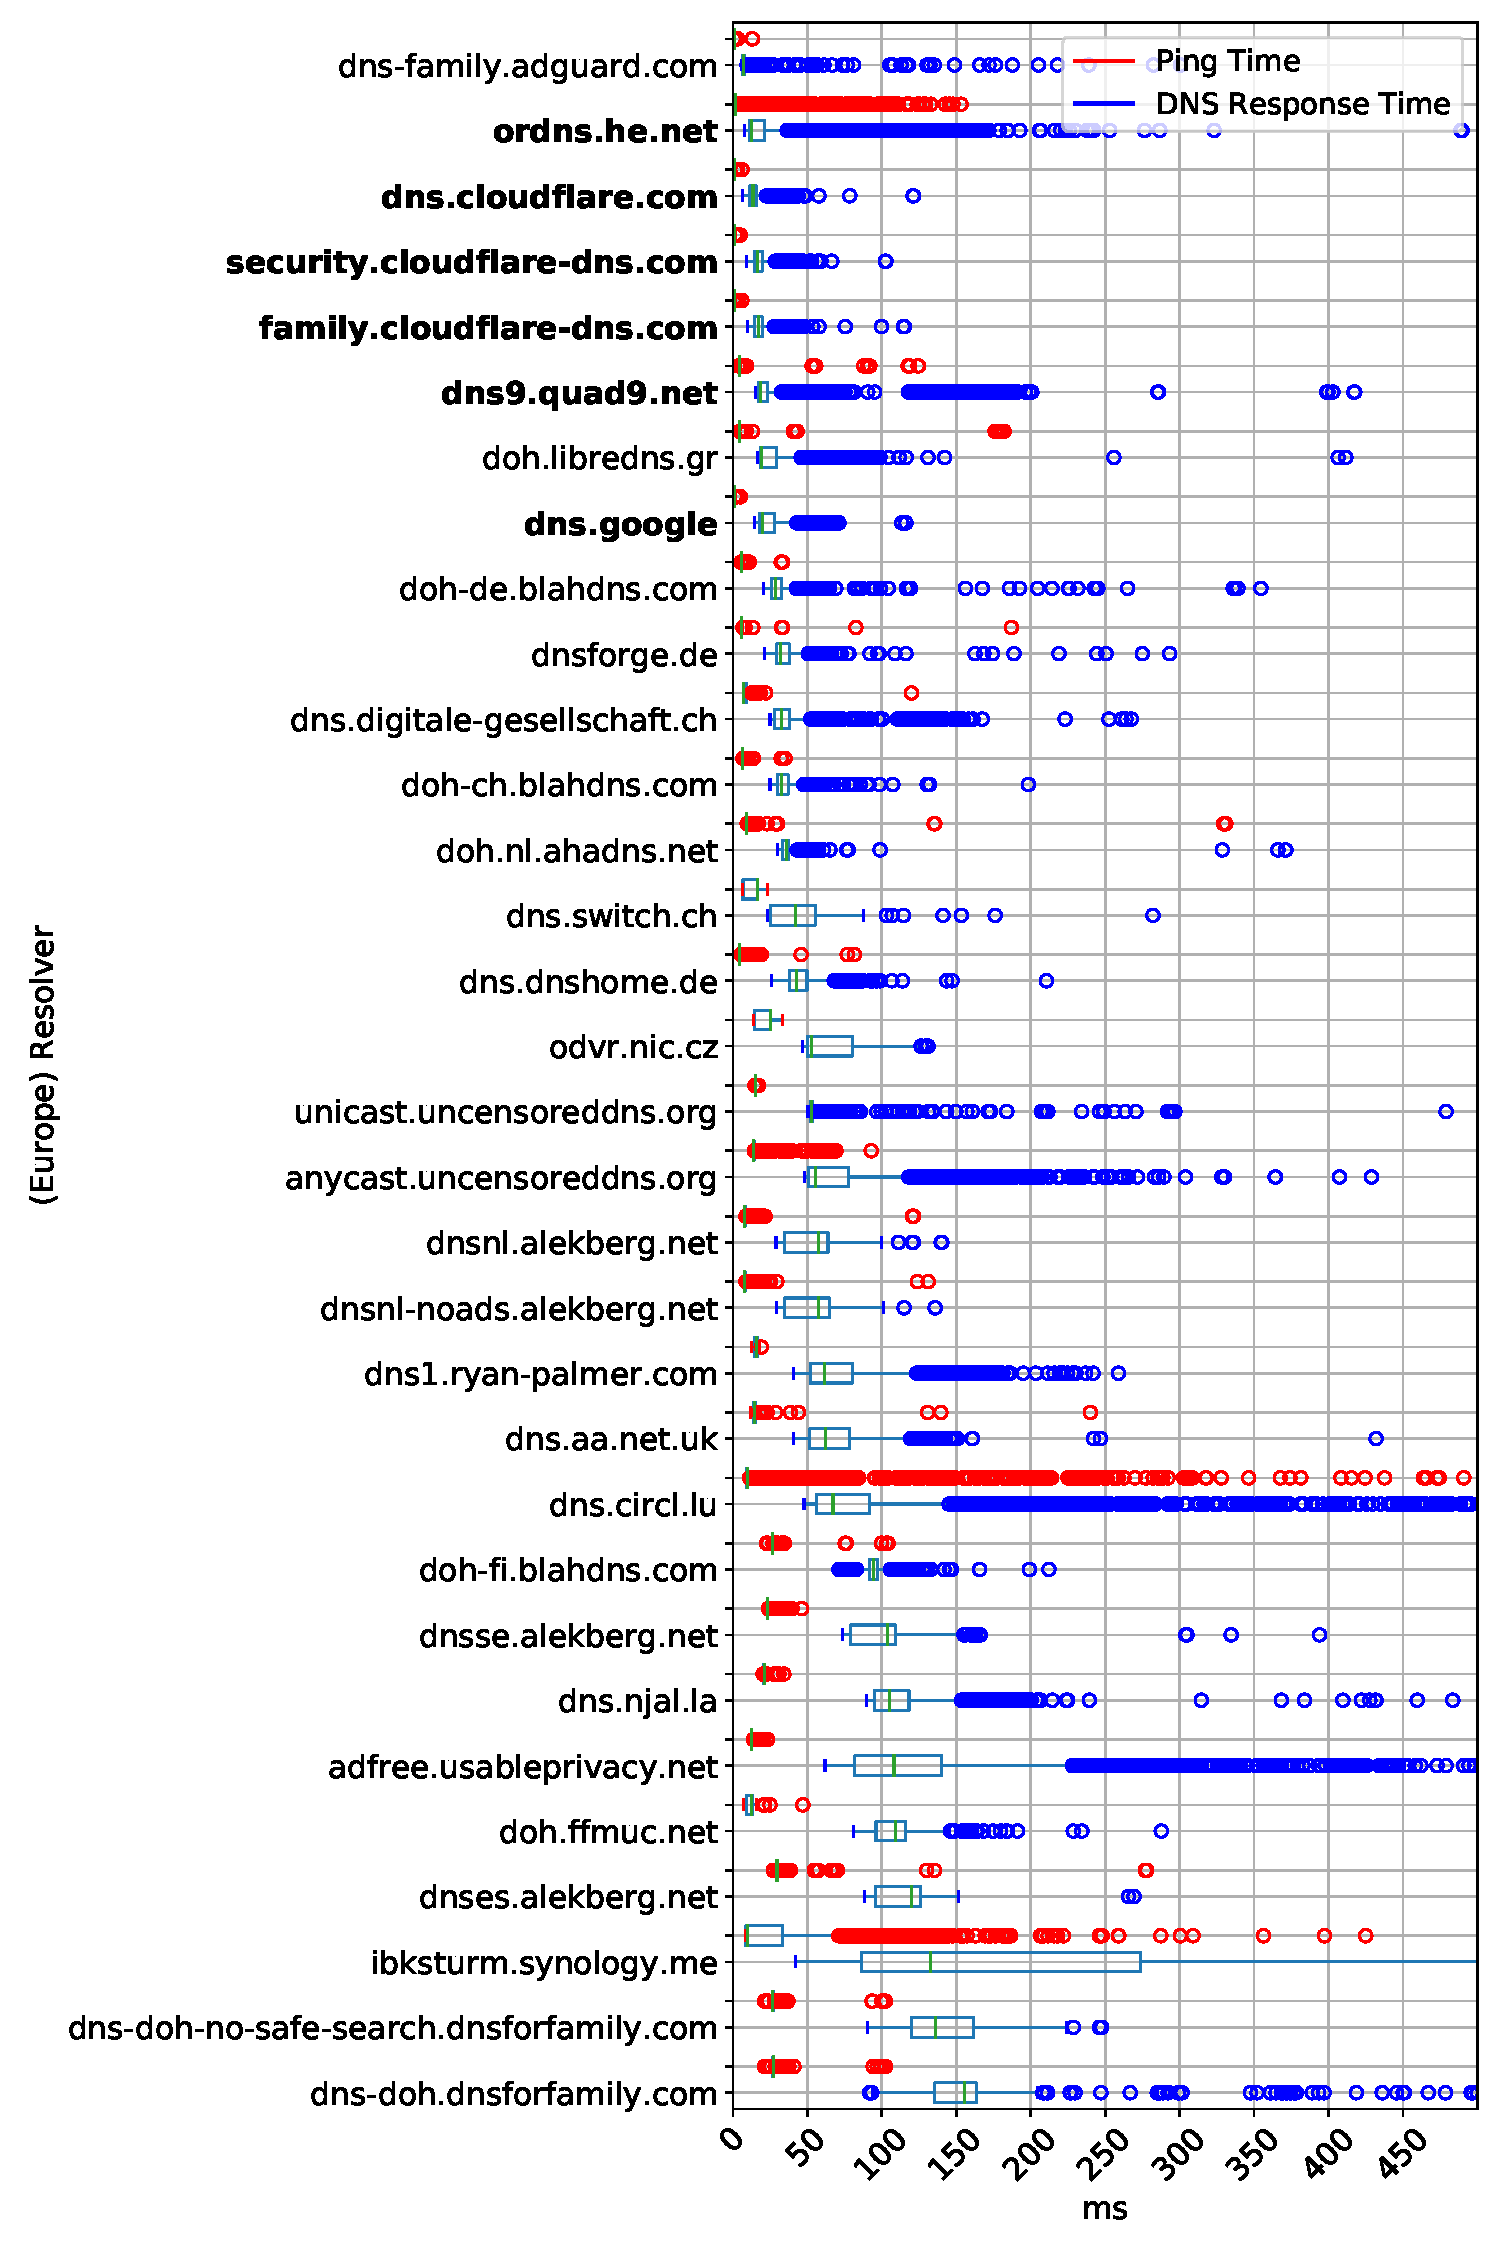
\includegraphics[width=0.32\linewidth]{figures/Frankfurt_Europe.pdf}}%
\caption{Local-to-local resolvers.}
\end{minipage}
\end{figure}
\fi


